% !TEX root =  ../Dissertation.tex

\chapter{Results and Discussion}

In this section, it is presented a series of experiments done in different RL environments. Particularly, a 31-state simple GridWorld was used as proof of concept to analyze the efficient of our method by evaluating three keys problems in non-uniform sampling methods, such as task-agnostic sampling, outdated priorities, and state space coverage. After exploring these main issues, a general evaluation on slightly more complex was done to measure the performance of our algorithm in the RL scenario.

\section{Grid World - Episode Reward}

Episode Reward and Cumulative Reward were initially chosen to indicate the performance during training of different DQN extensions. The full priority weighting (weight: 1.0) version was used for BPERcn and BPERaa alternatives, such that it only prioritizes with bisimulation distances and not td-error\footnote{Additionally, a sweep over the priority weights: 0.1, 0.25, 0.5, 0.75 and 1.0 was done, and the results are shown in the Appendixes \ref{}}. The algorithm was executed for 5 independent executions and the mean, min and max values (bottom and upper margin of shaded regions) per time steps are show in Figure \ref{fig:episode_cumulative_reward}. The methods DQN and DQN + MICO work as baseline to compare all other methods. 


Figure \ref{fig:episode_reward_grid_world} illustrates the episode reward per time steps during training, calculated in a 100 steps average window. While all methods show an improvement over time, converging after 100k steps, both BPERcn and BPERaa show promising improvements early in the training process, obtaining better performance than baselines and PER extension. However, over time, BPERaa keeps more consistent and stable improvements, indicating a better manage of priorities in the experience replay, while BPERcn shows a decrease of performance after the time step 30k. This results suggest that the smoother relative strategy 2, BPERaa, could in fact be beneficial in practice. Additionally, even though the GridWorld is a simple environment, the PER alternative under performs against all the other methods over time, showing the effectiveness of prioritizing behavioral dissimilar states.

The cumulative reward in Figure \ref{fig:cumulative_reward} helps us to check the overall time collected reward, a higher value will indicate a better ability to follow actions that leads to positive rewards. This complementary information indicates us that BPERaa in fact produces a policy that collect higher rewards, increasing the performance over the direct baseline DQN + MICO, which effectively show us that BPERaa is in fact making a positive effect in improving DQN + MICO. Alternatively, the other strategy, BPERcn, shows improvements in the earlier stages of learning, but eventually start decreasing the performance (around the 50k step) making the DQN + MICO reward acquisition worse, but keeping a similar performance that the baseline DQN. Overall, the PER alternative is the worse having difficulties to collect the rewards and in fact hindering the learning of the baseline DQN. 

\begin{figure}[h]
    \centering
    \begin{subfigure}{0.45\textwidth}
    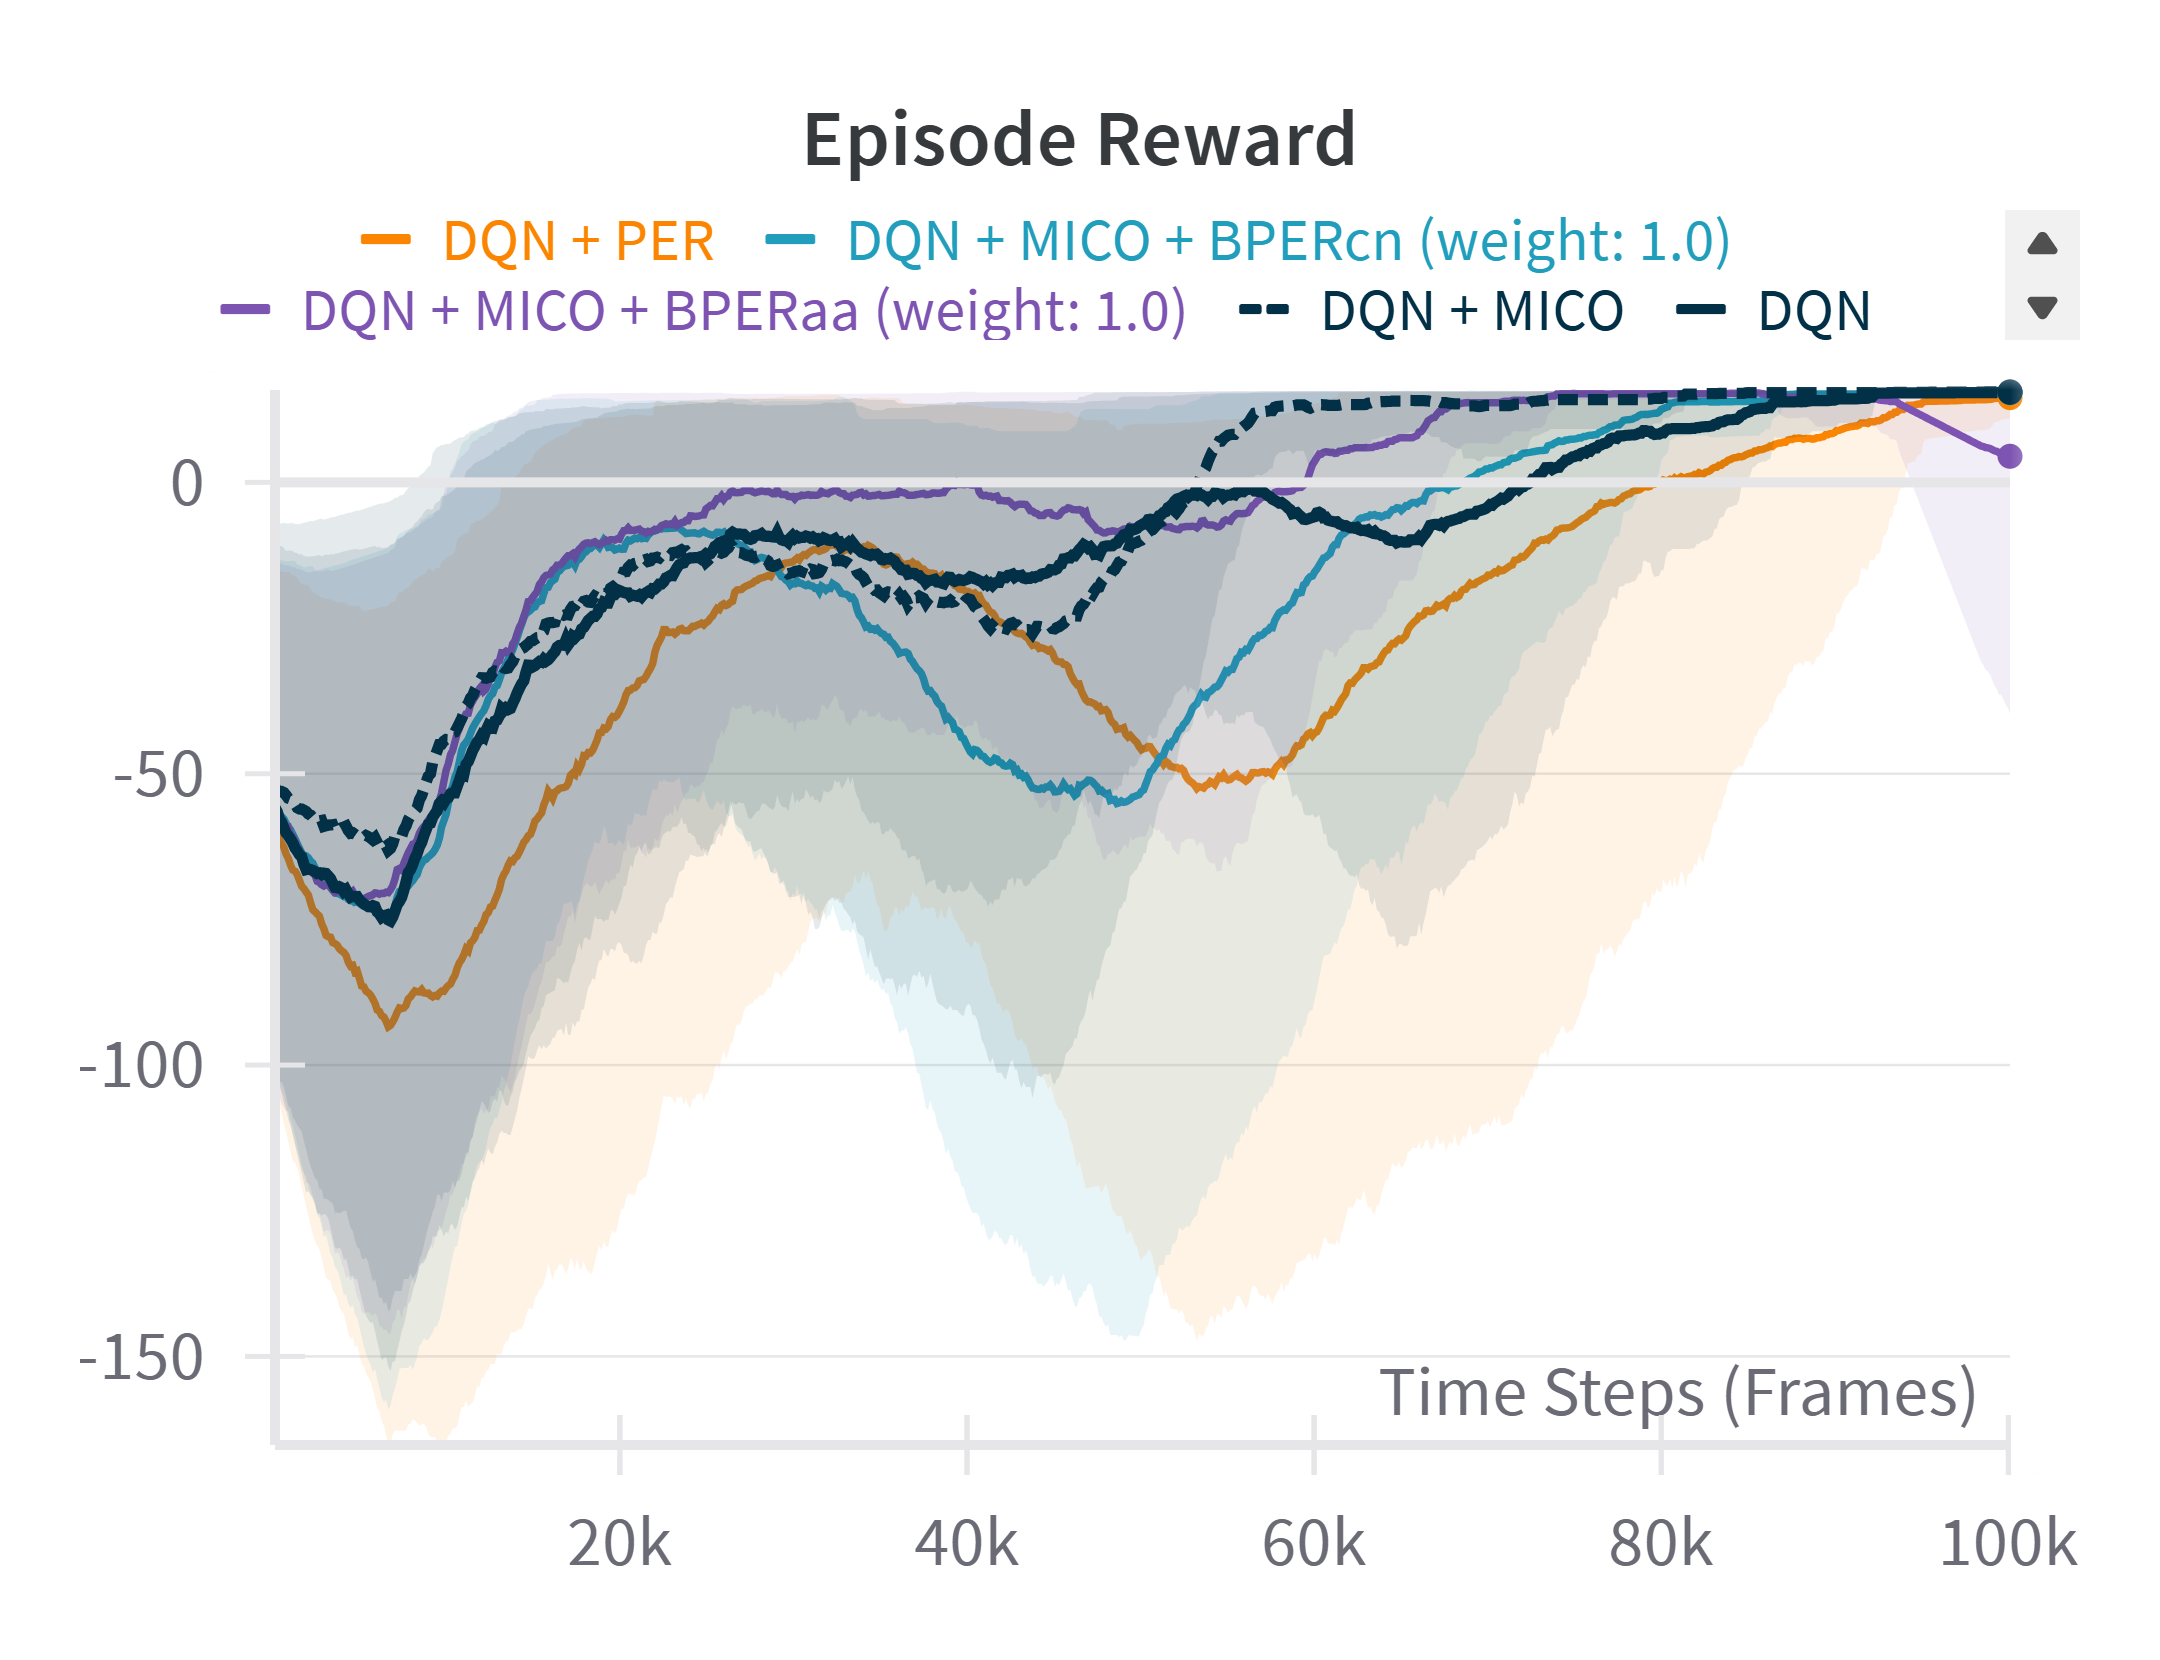
\includegraphics[width=\linewidth]{Results/grid_world/episode_reward_grid_world_window_100.png}
        \caption{Episode Reward}
        \label{fig:episode_reward_grid_world}
    \end{subfigure}
    \hfill
    \begin{subfigure}{0.45\textwidth}
        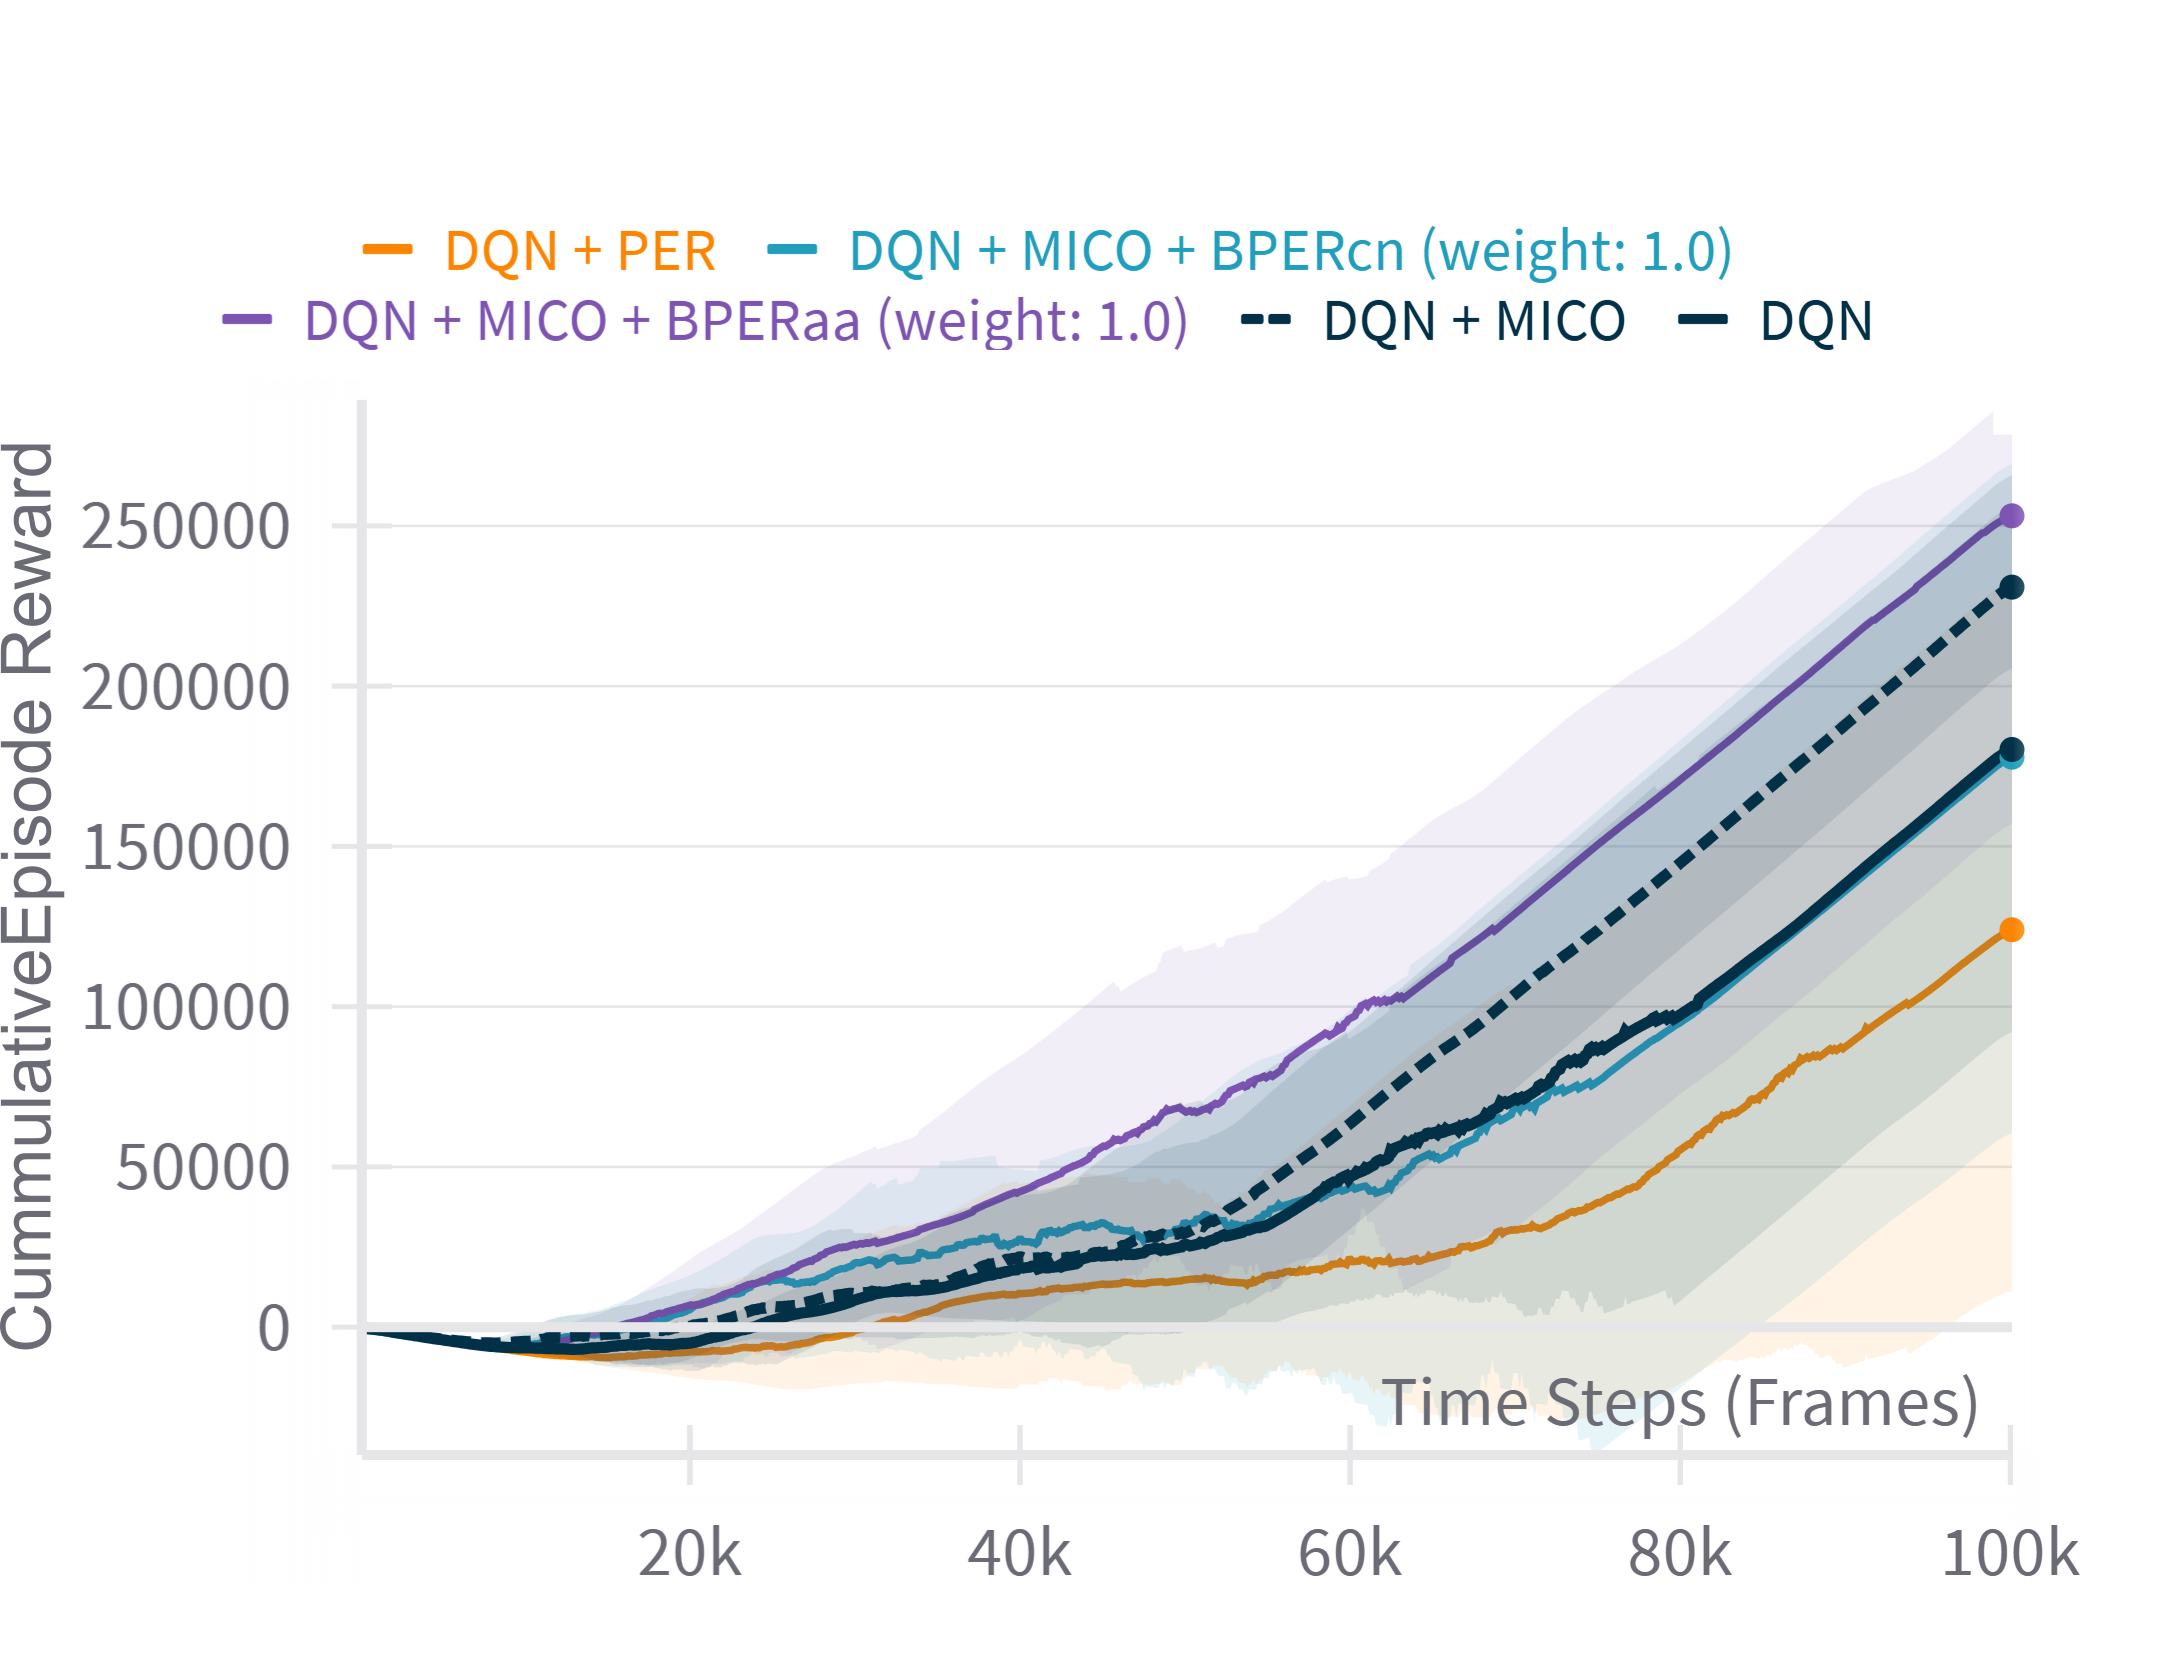
\includegraphics[width=\linewidth]{Results/grid_world/cumulative_episode_return.png}
        \caption{Cumulative Reward}
        \label{fig:cumulative_reward}
    \end{subfigure}
    \caption[Episode and Cumulative Reward]{\textbf{Episode and Cumulative Reward.} Reward performance comparison for different methods over time. The results represent the average from 5 independent executions, with shaded regions indicating the variability for each method.}
    \label{fig:cumulative_episode_reward}

\end{figure}


Exploring other perspective of the previous results, we proposed the episode reward gain to analyze more in detail the level of improvement of the proposed methods against our baselines (DQN and DQN + MICO). Figure \ref{fig:episode_reward_gain_dqn_and_mico} illustrates the Episode Reward gain on two different baselines, calculated on a window of 100 steps, and average over 5 independent executions. It is important to notice that only the mean values were used for the calculations. The results ratifies the excel improvements of BPERaa strategy over the other methods: BPERcn and PER againts both baselines, and showcases similar improvements of both bisimulation strategies in the earlier stages of the training. However, as mentioned before, this performance decreases in BPERcn around the step 30k. Under both baselines, the PER method underperform enormously by hinder the proper learning of the policy.

\begin{figure}[h]
    \centering
    \begin{subfigure}{0.45\textwidth}
    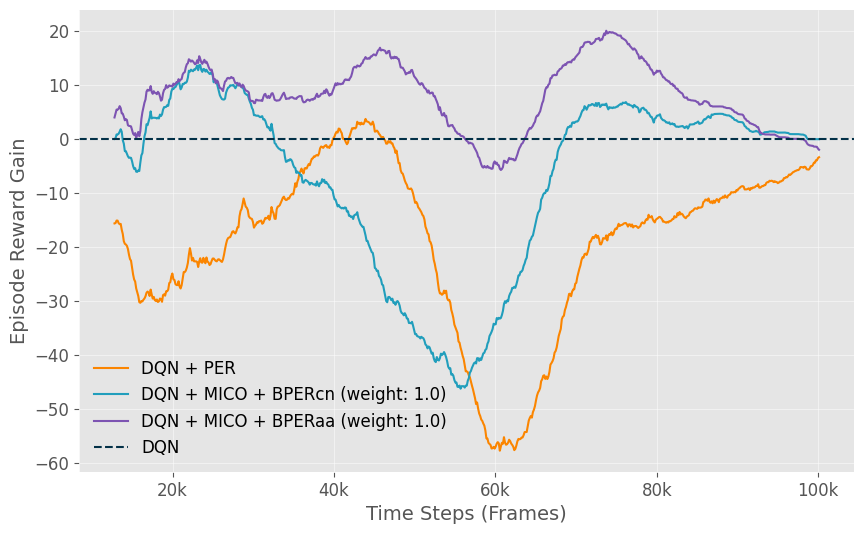
\includegraphics[width=\linewidth]{Results/grid_world/episode_reward_gain_baseline_dqn.png}
        \caption{Baseline DQN}
        \label{fig:episode_reward_gain_dqn}
    \end{subfigure}
    \hfill
    \begin{subfigure}{0.45\textwidth}
        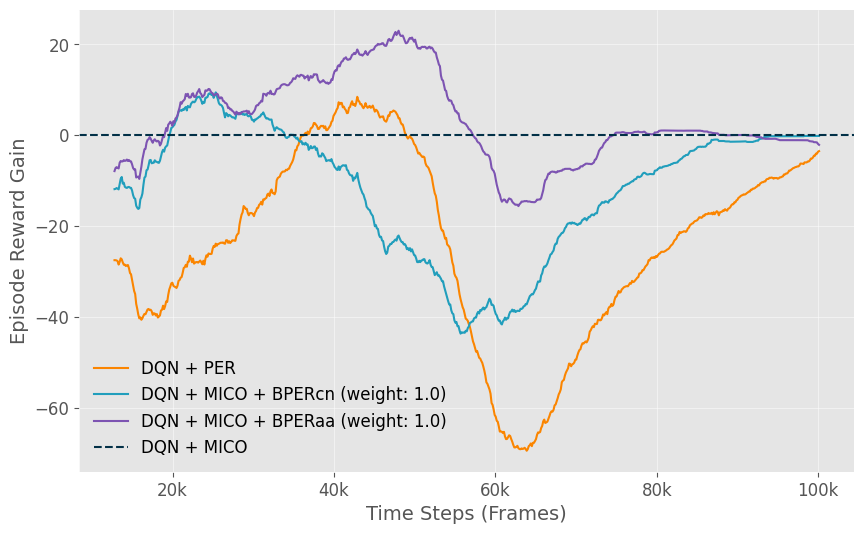
\includegraphics[width=\linewidth]{Results/grid_world/episode_reward_gain_baseline_dqn_mico.png}
        \caption{Baseline DQN + MICO}
        \label{fig:episode_reward_gain_dqn_mico}
    \end{subfigure}
    \caption{Episode Reward Gain }
    \label{fig:episode_reward_gain_dqn_and_mico}
\end{figure}

\section{Task-agnostic Sampling}

In this section, the intention is empirically demonstrate that the proposed method takes into account the behavior for prioritized samples efficiently. To do that, we require a way to quantitatively evaluated how many behavioral dissimilar transitions there are in the current experience replay. Specifically, the on-policy bisimulation recurrent operator $T_K^\pi$ for deterministic environments (see Equation \ref{eq:deterministic_on_policy_bisimulation_metric}) allow us to calculate exact on-policy bisimulation distances. Then, each transition in the experience replay can be associated with a exact bisimulation distance between the current and next state, effectively providing a behavioral value indicator per transition, and allowing us to evaluate the level of behavioral similar or dissimilar transitions in an experience replay. 

Figure \ref{fig:exact_bisimulation_distributions} illustrates the distribution over those exact current-next on-policy bisimulation distances in the experience replay over time, with the last distribution (100k) highlighted on top of the figure. In the strategies BPERcn and BPERaa, the behavioral dissimilar transitions evolve to larger values than PER over time, specifically exact bisimulation distance higher than 30 and between 15 and 20 are more frequent in the experience replay. It clearly demonstrates how our method will prioritized more frequently those larger behavioral dissimilar transitions. As the BPERcn encourages highly dissimilar transition between the current and next states approximated in the loop, the results from Figure \ref{fig:exact_bisim_bpercn} are expected. However, a more interesting result is that despite of BPERaa prioritized the transition based on a relative priority to the current mini-batch, this second strategy is still able to prioritize dissimilar experience as efficiently as the strategy BPERcn (see Figure \ref{fig:exact_bisim_bperaa}).

Another interesting result is that even though the methods aim to prioritized highlight dissimilar transitions, Figures \ref{fig:exact_bisimulation_distributions} still show a lot of transitions with exact bisimilar distance close to zero, possible coming from the nature of the environment that contains highly similar states. Another thing that could be influenced this result is the use of a large buffer of 100000, set deliberately with a large capacity to contrast behaviors under large scales circumstances which are more common in practice with stated-of-the-art methods.

\begin{figure}[h]
    \centering
    \begin{subfigure}{0.32\textwidth}
    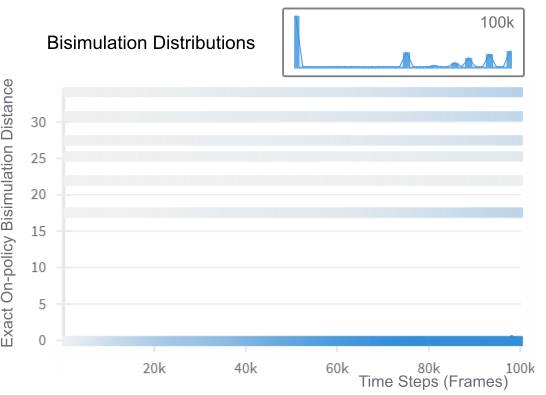
\includegraphics[width=\linewidth]{Results/grid_world/exact_bisimulation_dqn_per.png}
        \caption{DQN + PER}
        \label{fig:exact_bisim_per}
    \end{subfigure}
    \hfill
    \begin{subfigure}{0.32\textwidth}
        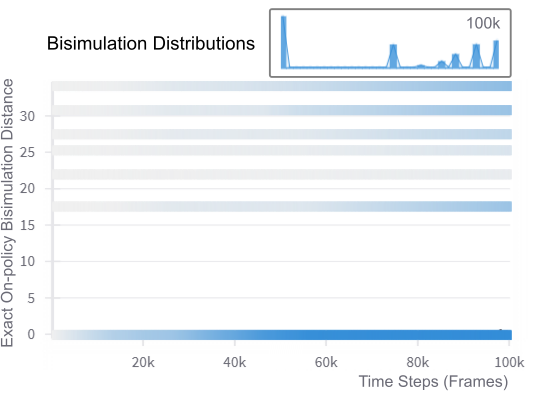
\includegraphics[width=\linewidth]{Results/grid_world/exact_bisimulation_dqn_mico_bpercn.png}
        \caption{DQN (MICO) + BPERcn}
        \label{fig:exact_bisim_bpercn}
    \end{subfigure}
    \hfill
    \begin{subfigure}{0.32\textwidth}
        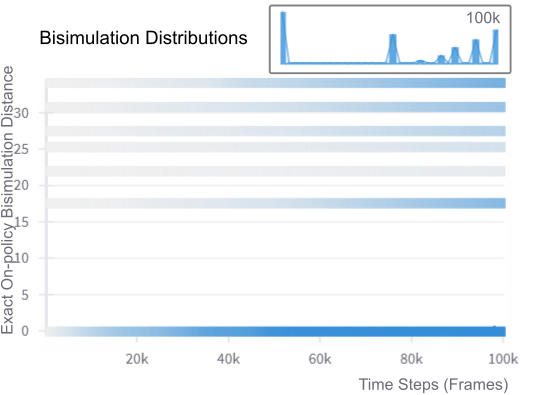
\includegraphics[width=\linewidth]{Results/grid_world/exact_bisimulation_dqn_mico_bperaa.png}
        \caption{DQN (MICO) + BPERaa}
        \label{fig:exact_bisim_bperaa}
    \end{subfigure}
    \caption{Two images side-by-side}
    \label{fig:exact_bisimulation_distributions}
\end{figure}

Now, we have an understanding of the amount of behavioral dissimilar transition, and an interesting point to analyze is how much of those transitions in the replay actually corresponds to high priorities values. To check that, Figure \ref{fig:priority_distributions} illustrates the evolution of priority distributions on the experience replay over time, with the last distribution (100k) high-lighted on top. Figure \ref{fig:priority_distribution_per} indicates an accumulation of low values priorities over time in the PER method, and with few larger priorities. Even though most of the priorities values are really low, they all together can occupy a large priority area, prioritizing or weighting transitions with low td-error more frequently, and consequently hindering the DQN learning; explaining the defficient in episode reward explored in previous experiments.

In contrast, both proposed strategies, BPERcn and BPERaa, generate consistently higher priorities over time, encouraging more behavioral dissimilar transitions. With BPERaa showing a slight higher variability in Figure \ref{fig:priority_distribution_bperaa}. Although these results do not associated dirrectly each priority value with the exact bisimulation distances mentioned before, it provides an idea of how many transition in the experience replay that are behavioral dissimilar are actually being prioritized over time.

\begin{figure}[h]
    \centering
    \begin{subfigure}{0.32\textwidth}
    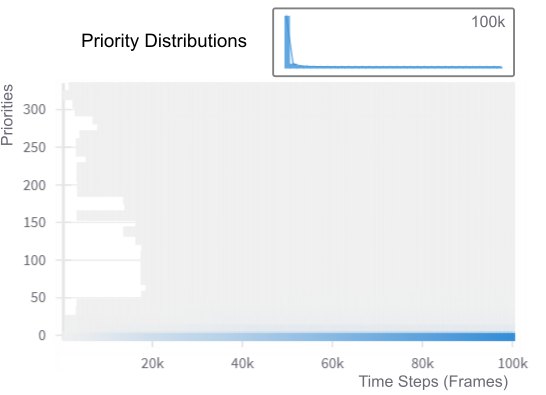
\includegraphics[width=\linewidth]{Results/grid_world/priority_distribution_dqn_per.png}
        \caption{DQN + PER}
        \label{fig:priority_distribution_per}
    \end{subfigure}
    \hfill
    \begin{subfigure}{0.32\textwidth}
        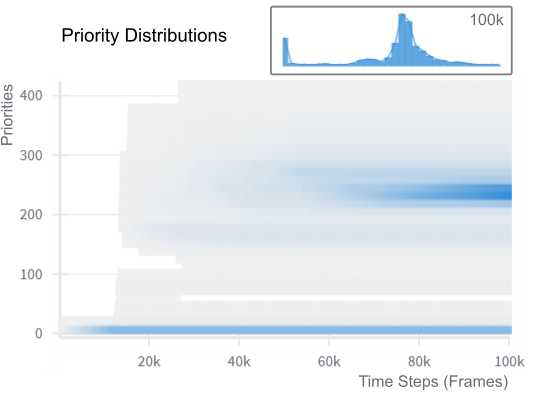
\includegraphics[width=\linewidth]{Results/grid_world/priority_distribution_dqn_mico_bpercn.png}
        \caption{DQN (MICO) + BPERcn}
        \label{fig:priority_distribution_bpercn}
    \end{subfigure}
    \hfill
    \begin{subfigure}{0.32\textwidth}
        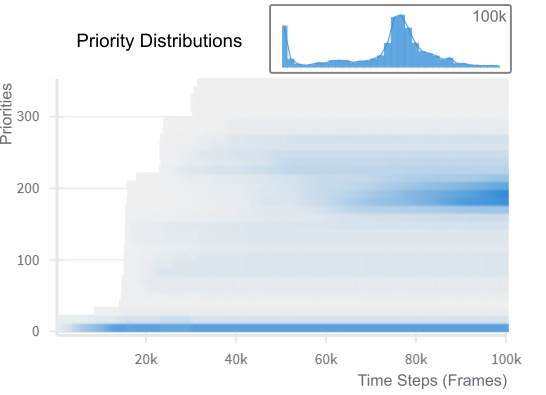
\includegraphics[width=\linewidth]{Results/grid_world/priority_distribution_dqn_mico_bperaa.png}
        \caption{DQN (MICO) + BPERaa}
        \label{fig:priority_distribution_bperaa}
    \end{subfigure}
    \caption{Two images side-by-side}
    \label{fig:priority_distributions}
\end{figure}


Later, Figure \ref{fig:quartiles_all_methods} show a qualitative visual inspection of the frames corresponding to the main quartiles priorities values in the experience replay in the time step 90k. The low quartiles (min, 25\%) corresponds to frames with low sampling probability, and higher quartiles (75\% and max) corresponds to frames with higher sampling probability. The top row corresponds to the current states and the bottom row corresponds to the next states in each transition. Figure \ref{algorithm:dqn_per} exhibits the aforementioned difficulties of PER method when trying to prioritized state transitions using the td-error. In the quartile 25\% transition, the algorithm assigns low value priority to a transition that reach the goal, while assign high priority in the quartile 75\% to a transition that gets stuck in the same position without reaching the goal; clearly leading to a low expected learning progress. On the contrary, the strategies BPERcn and BPERaa show a consistencies along the low quartiles by keeping lower priorities to transition that get stuck or going backwards with the goal, while keeping higher priorities to transition that moves towards the goal in the high quartiles. Notice, however, it seems to be small variances, specially in BPERcn where in the quartile 25\% we can see a lower transition probability assigned to a transition that leads towards the goal; suggesting scarce high priorities problems. For reference an additional visual inspection of the quartiles in the time step 50k is show in the Appendix \ref{}. 

% Notice that we could allegate that the low prioritization of the two quartiles makes sense because they could be associated with a small td-error; however, this is not necessarily true. In fact, accorsing previous Figure \ref{fig:episode_reward_grid_world}, there is still room for learning in the time step 90k for the DQN + PER algorithm.

\begin{figure}[h]
    \centering
    \begin{subfigure}{1.\textwidth}
    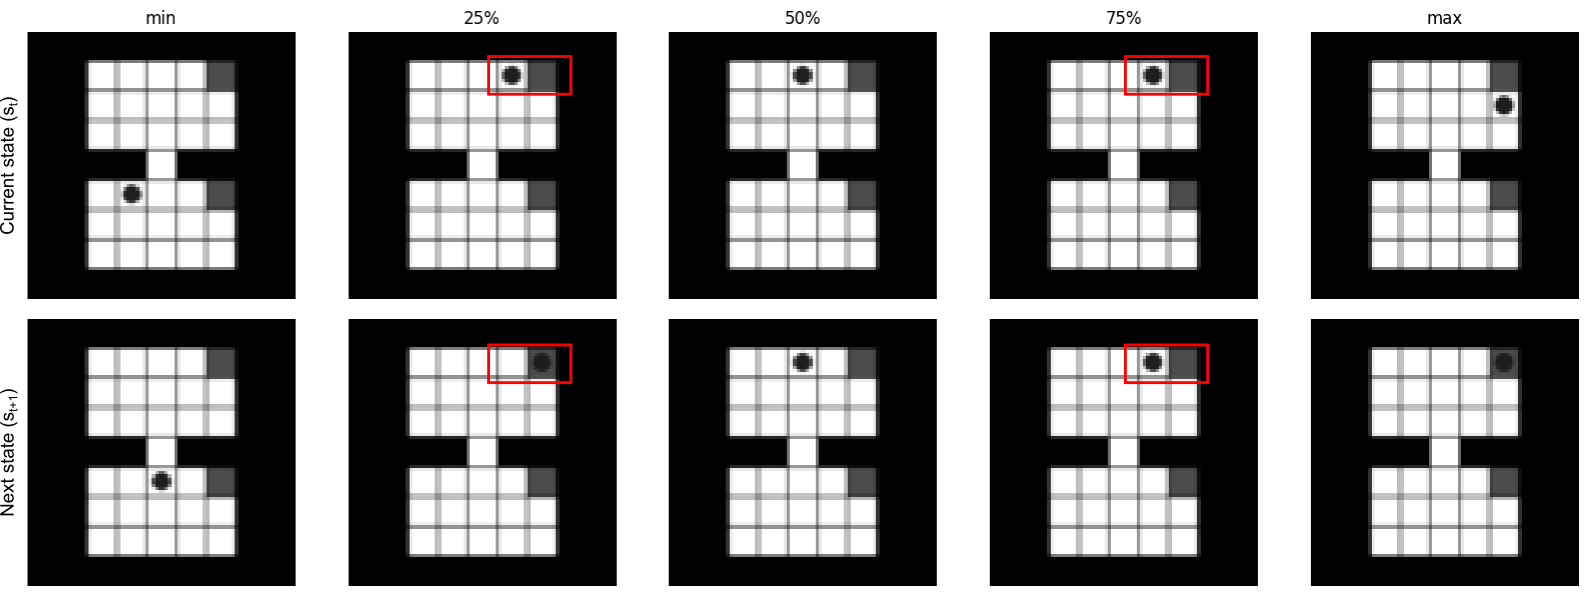
\includegraphics[width=\linewidth]{Results/grid_world/quartiles_images_per.png}
        \caption{DQN + PER}
        \label{fig:quartiles_per}
    \end{subfigure}
    \hfill
    \begin{subfigure}{1.\textwidth}
        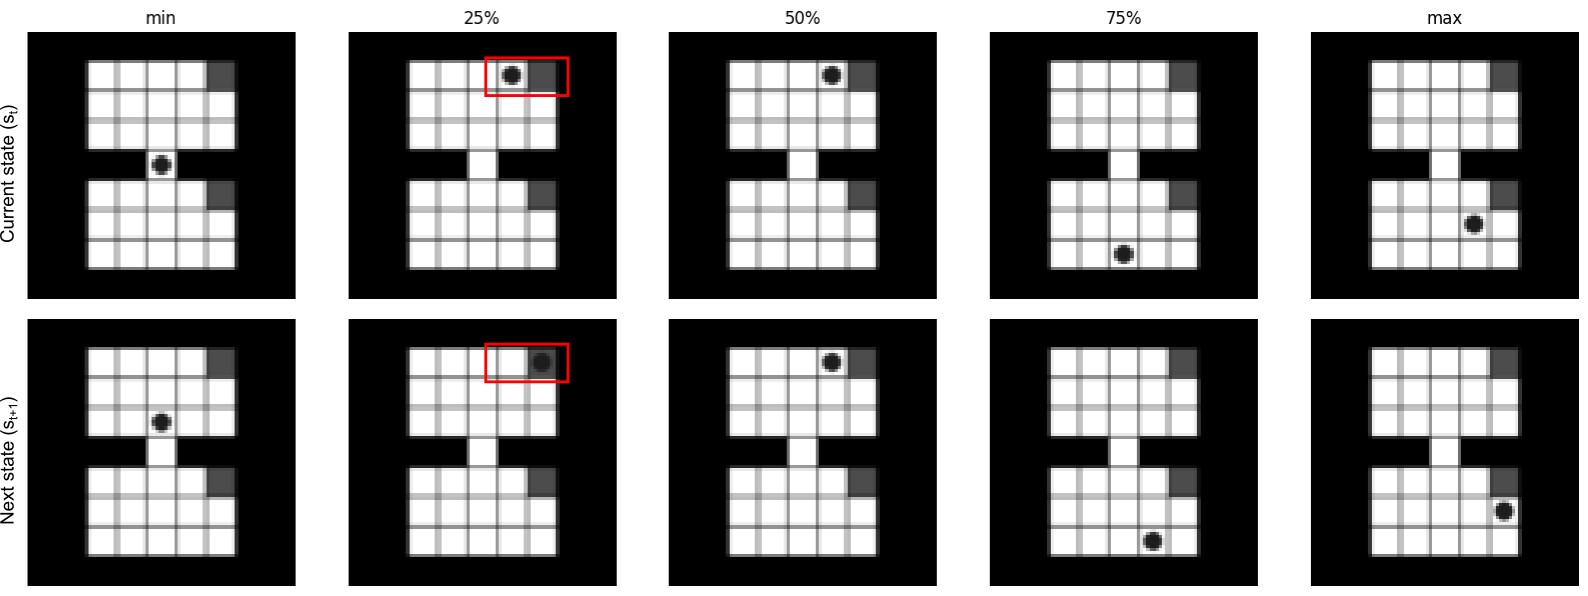
\includegraphics[width=\linewidth]{Results/grid_world/quartiles_images_dqn_mico_bpercn.png}
        \caption{DQN (MICO) + BPERcn}
        \label{fig:quartiles_bpercn}
    \end{subfigure}
    \hfill
    \begin{subfigure}{1.\textwidth}
        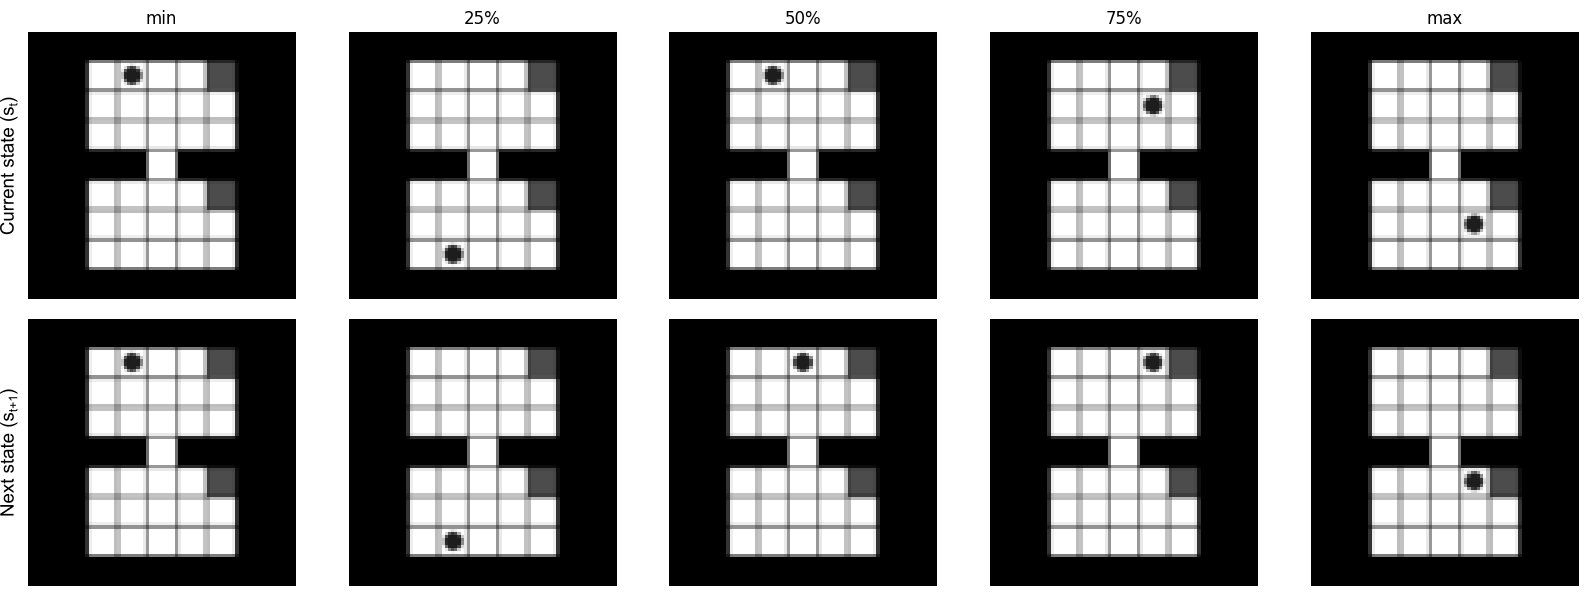
\includegraphics[width=\linewidth]{Results/grid_world/quartiles_images_dqn_mico_bperaa.png}
        \caption{DQN (MICO) + BPERaa}
        \label{fig:quartiles_bperaa}
    \end{subfigure}
    \caption{Two images side-by-side}
    \label{fig:quartiles_all_methods}
\end{figure}

The results in this section suggest that despite of the td-error is an indicator of possible improvement over the q-values, this is not enough to define a proxy of the expected learning progress in special scenario, where a notion of behavioral similarity works better as an indicator of expected learning progress.

\section{Outdated Priorities}

In this section, the intention is empirically demonstrate that the proposed method alleviate the oudated priorities method. Recall that the outdated priorities is a problem that happens due the way that the priorities are updated only in the current minibach, instead of updating the priorities in the whole experience replay or even better the whole state space. As we are not updating all the priorities, the priorities will be outdated leading to sampling probabilities with certain variabilities. In this experiment, we are measuring that level of variability by comparing the distance between the ideal priority distribution (when priorities are updated in the whole state space under the current policy) vs the approximated sampling priority of the experience replay, as mentioned in Section \ref{sec:experimental_setup}

Figures \ref{fig:priority_dist_distance_on_policy_weighting} and \ref{fig:priority_dist_distance_uniform_weighting} show the on-policy and uniform weighting schemes respectively for calculating the distance between the aforementioned distributions, taken in average over 5 independent executions over time. The PER method exhibits a higher distances over time than the strategies BPERcn and BPERaa; even showing less variability among executions. Although our method does not provides distances close to zero (such as Pan et al.'s work \cite{pan2022understanding}) indicating a perfect match between distributions, our method reduce and alleviate significantly the difference between the distributions without relying on extract model-based assumptions. 

\begin{figure}[h]
    \centering
    \begin{subfigure}{0.45\textwidth}
    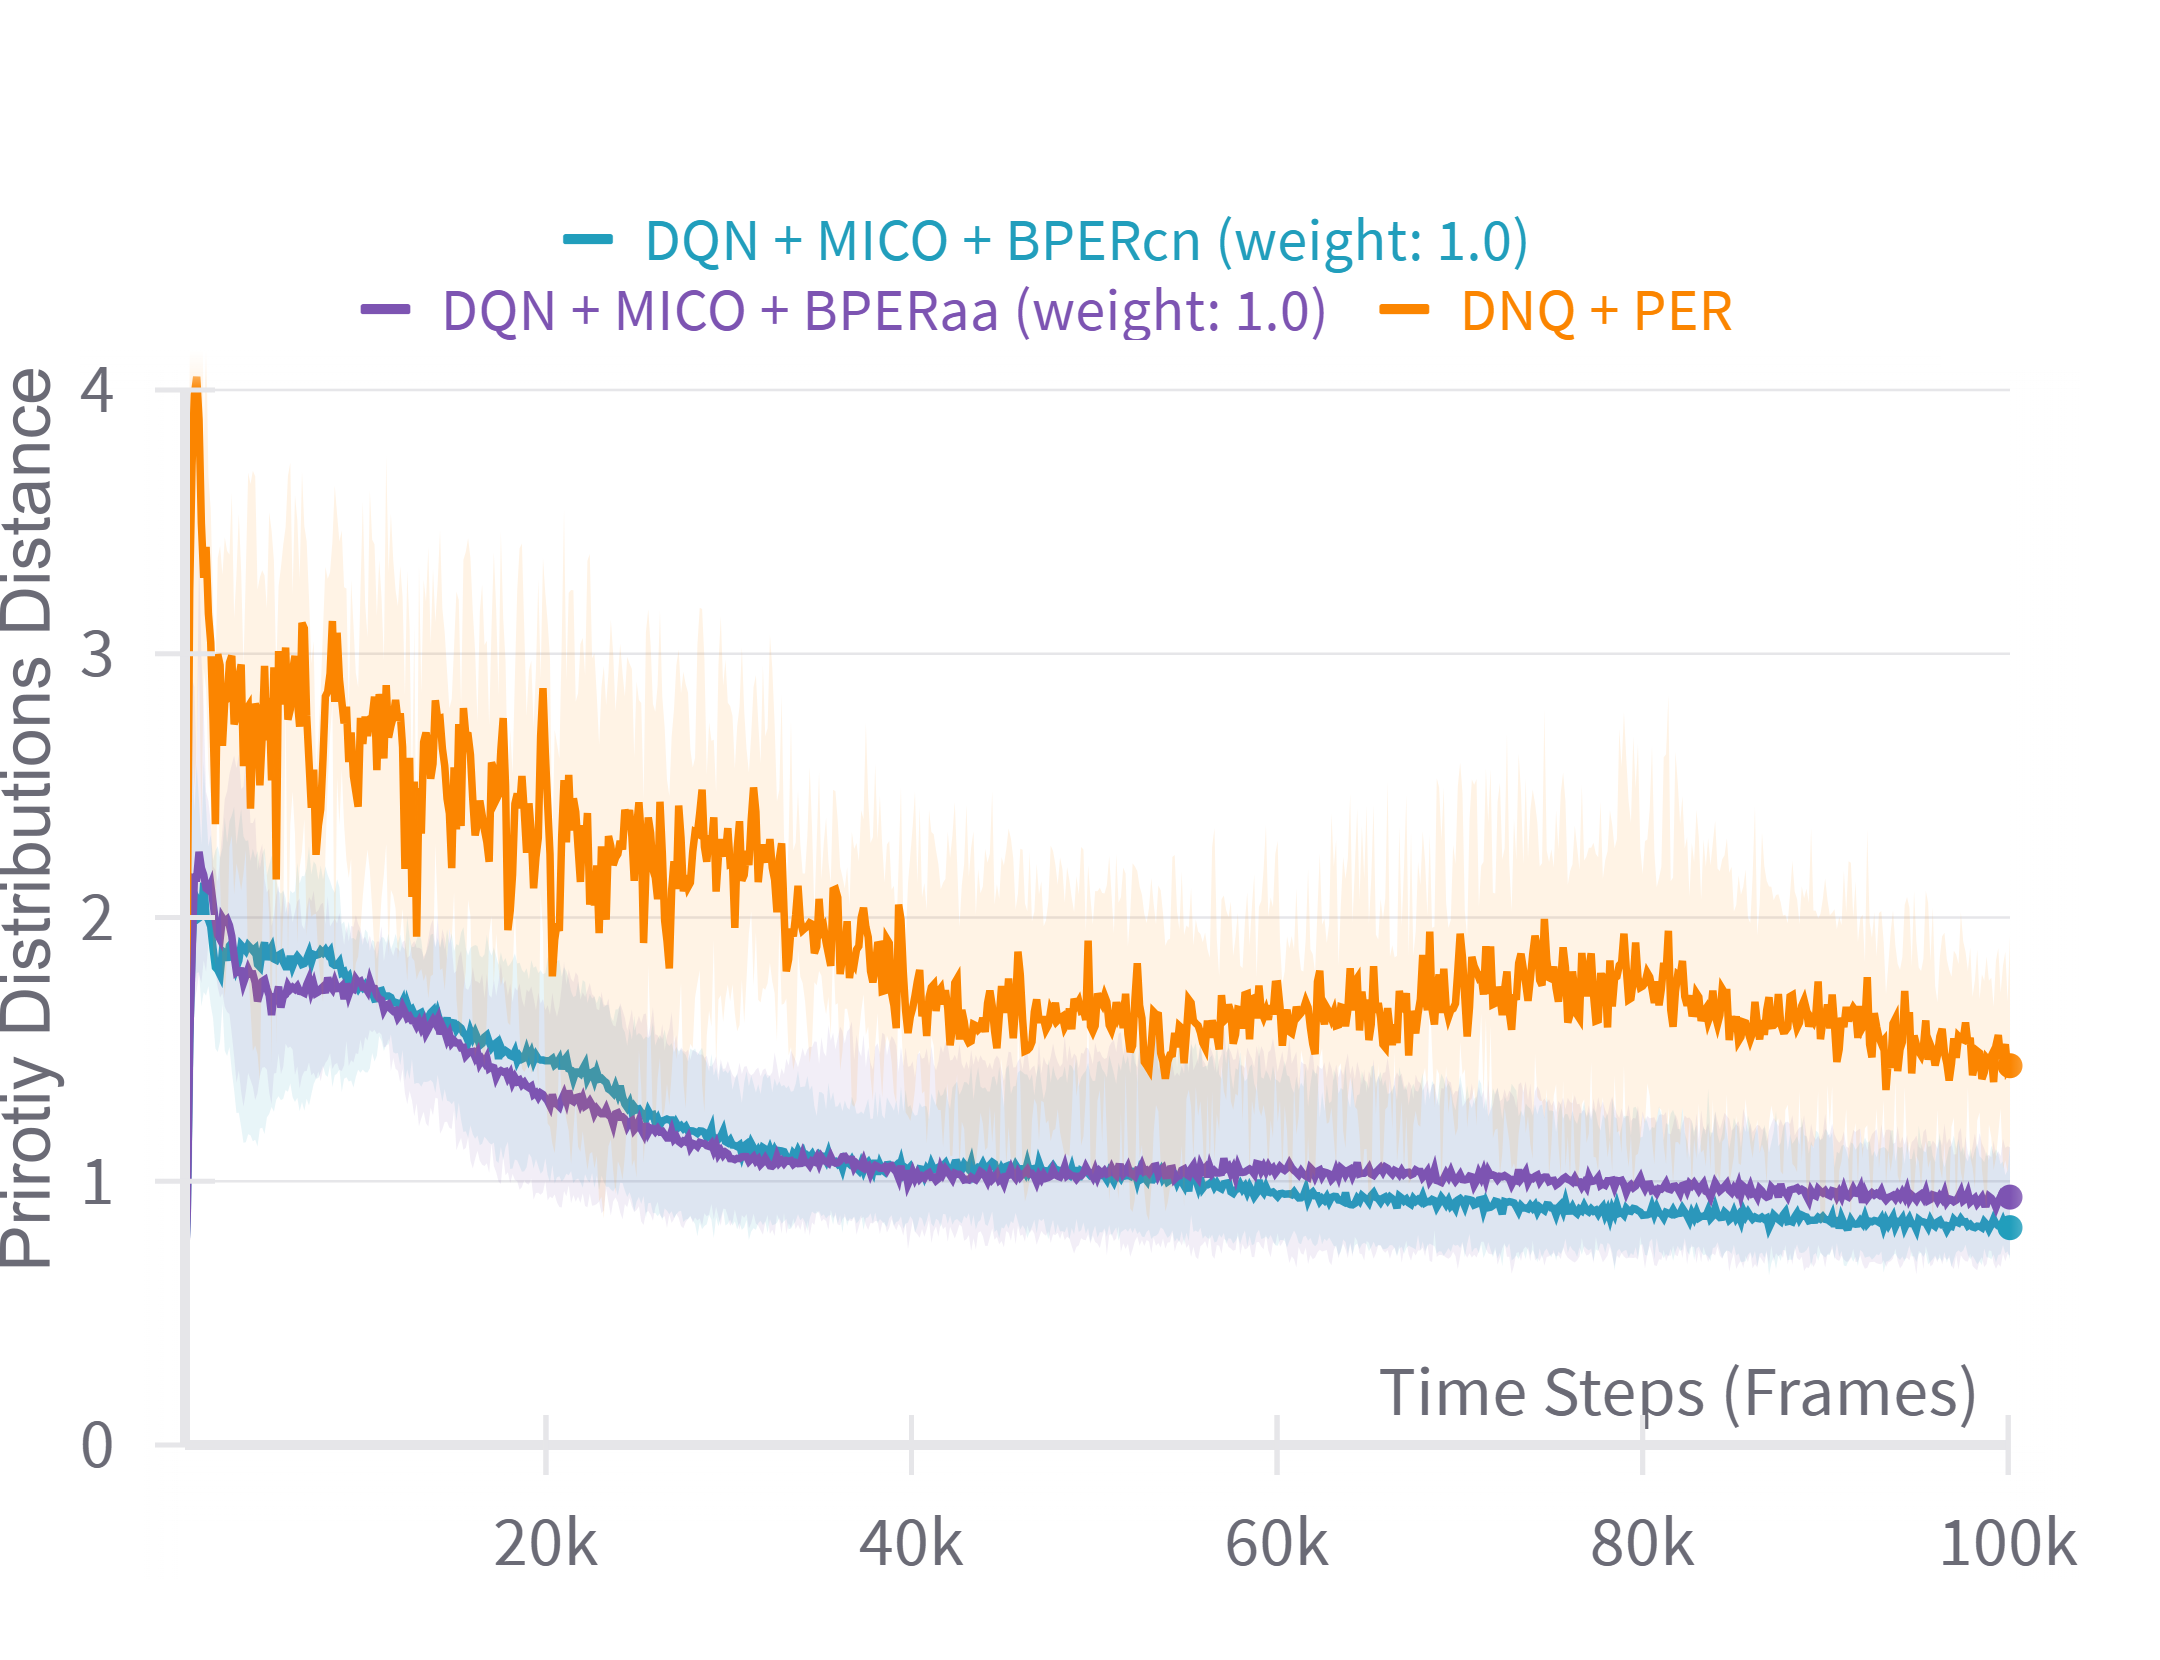
\includegraphics[width=\linewidth]{Results/grid_world/on_policy_weighting_outdated_priorities.png}
        \caption{On-policy Weighting}
        \label{fig:priority_dist_distance_on_policy_weighting}
    \end{subfigure}
    \hfill
    \begin{subfigure}{0.45\textwidth}
        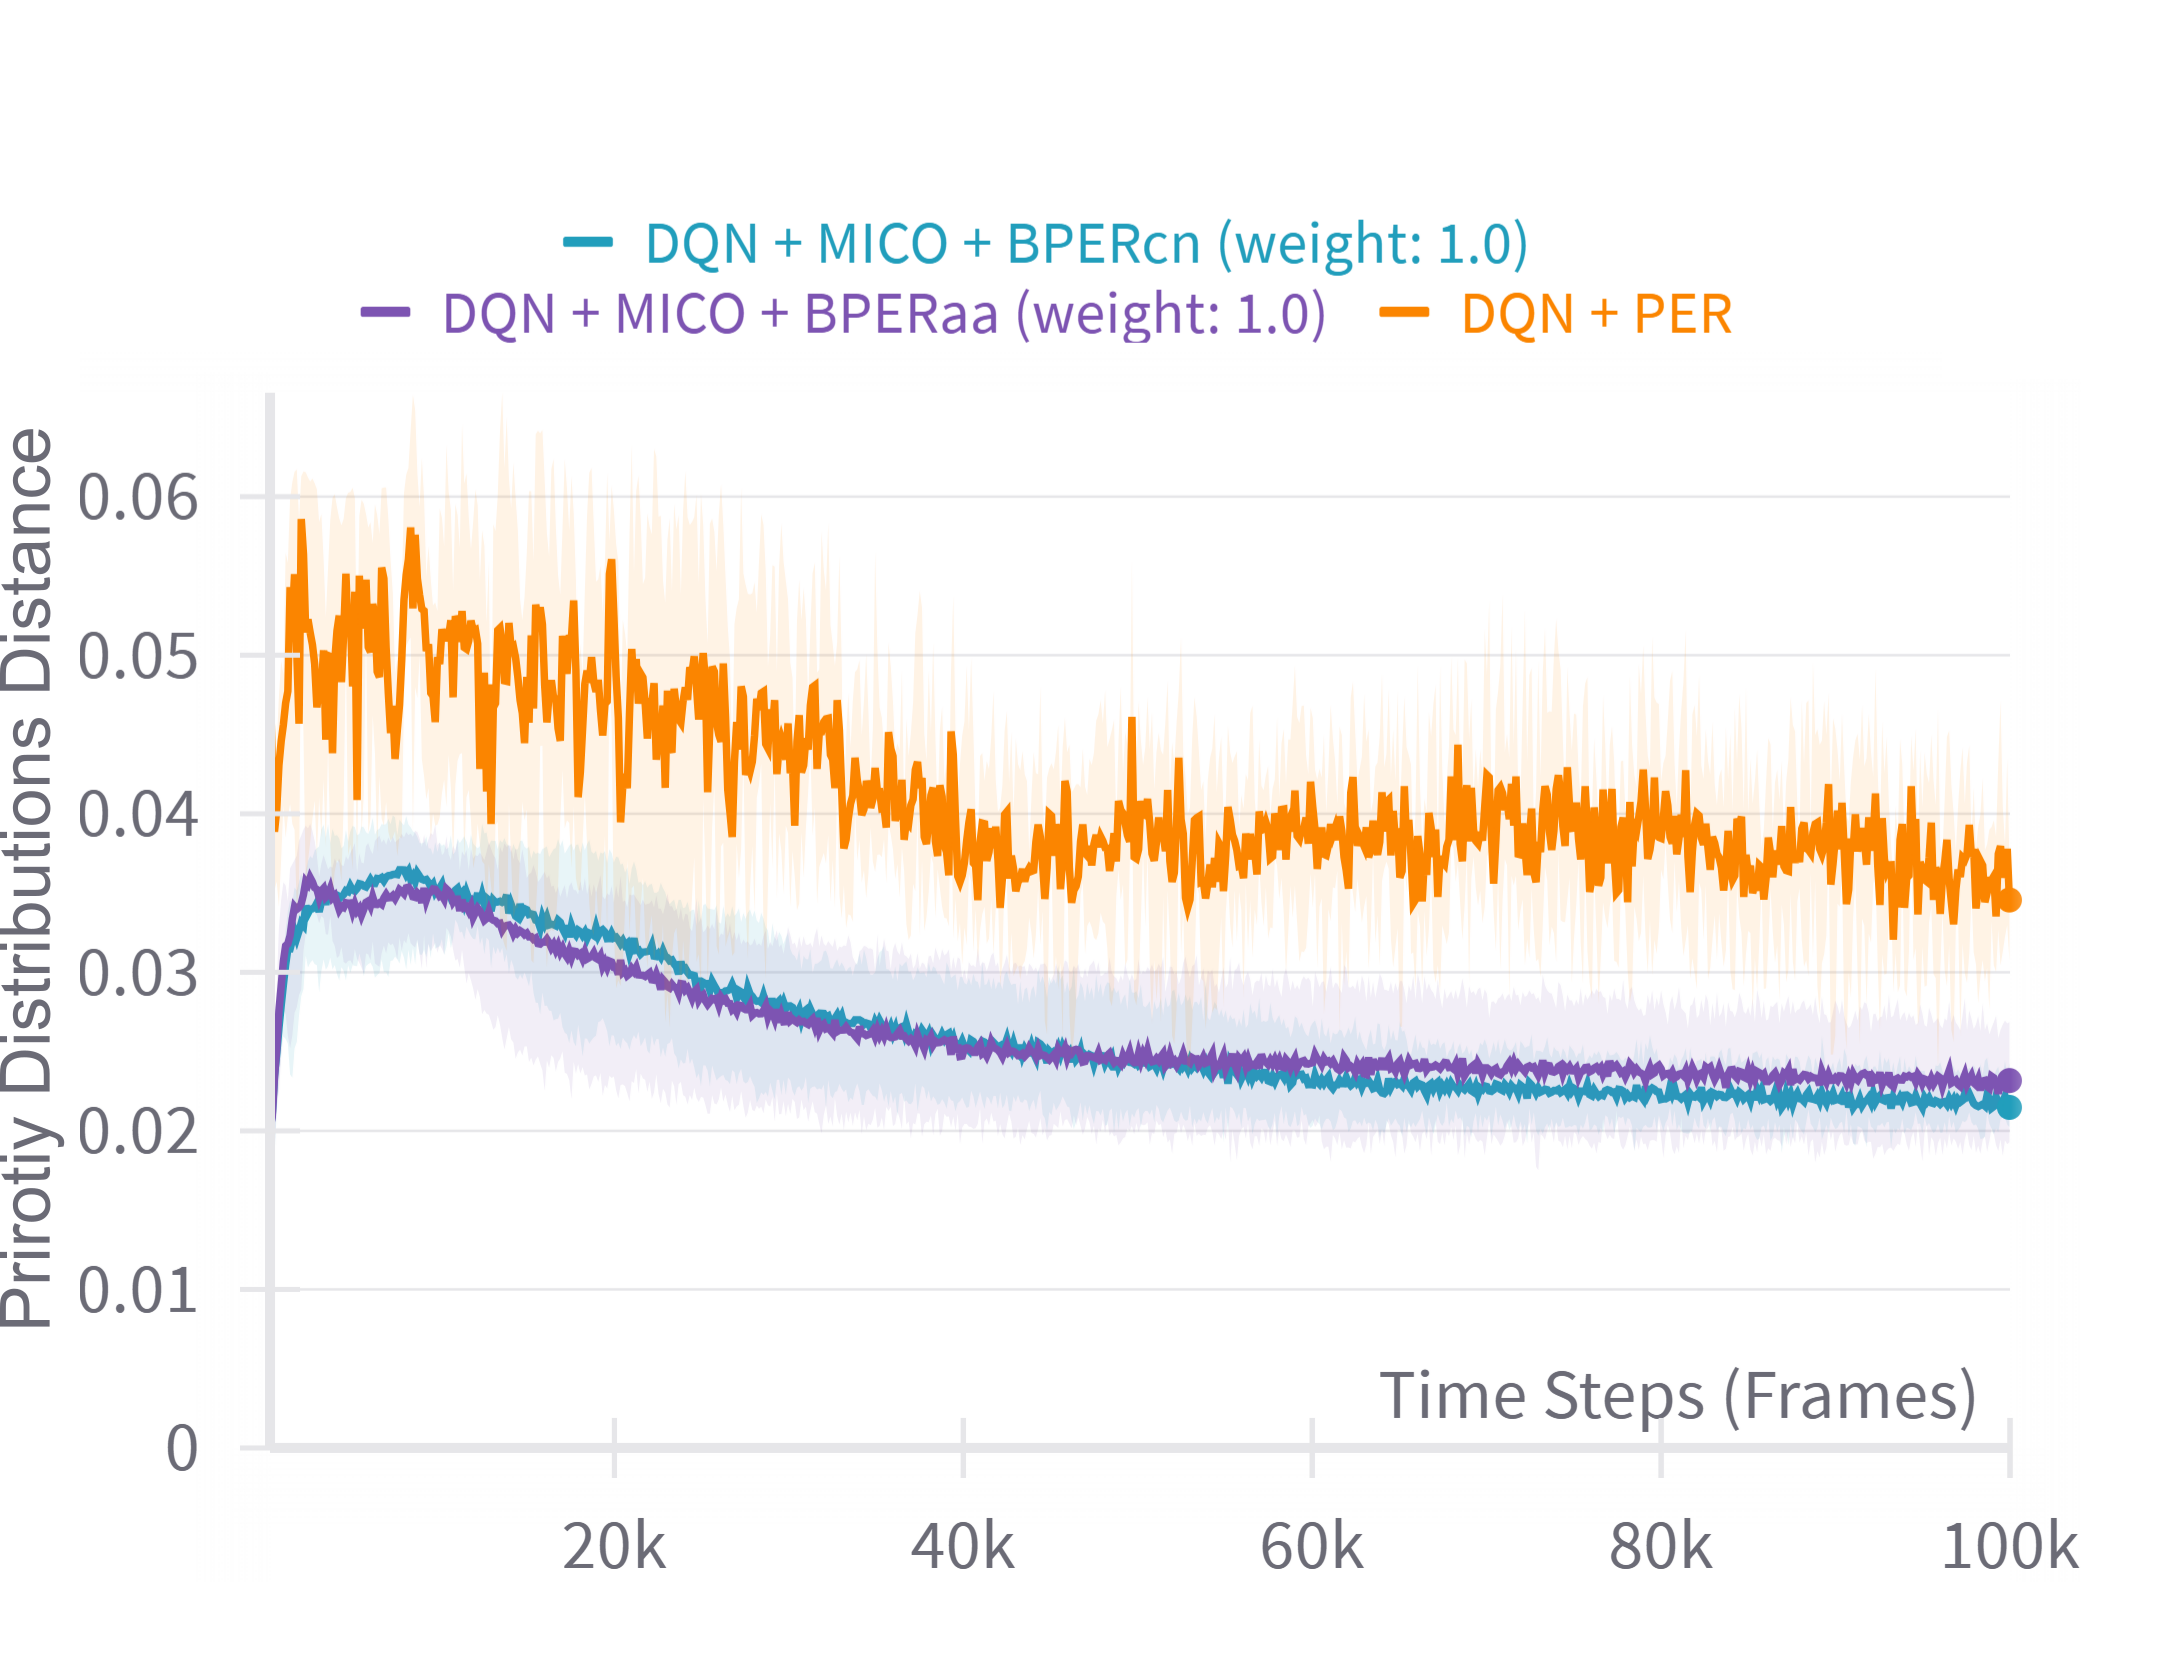
\includegraphics[width=\linewidth]{Results/grid_world/uniform_weighting_outdated_priorities.png}
        \caption{Uniform Weighting}
        \label{fig:priority_dist_distance_uniform_weighting}
    \end{subfigure}
    \caption{Two images side-by-side}
    \label{fig:priority_dist_distance}
\end{figure}

\section{State Space Coverage}

In this section, the intention is empirically evaluated that our approach address the state space coverage problem. The state coverage is related with the lack of visiting states because the experience replay only captures a given number of possible states. It is an exploration problem and we evaluated it accordingly.

Figure \ref{fig:visitation_distributions} shows the state visitation distribution on the 31-state Grid World, where cell values corresponds to the count of visiting those states. The results indicates that the strategies BPERcn and BPERaa indeed confer a better exploration on the environment by visiting all states more frequently; with BPERcn performing slightly better than BPERaa. The DQN + MICO baseline outperforms DQN, and DQN + PER methods, by increasing the exploration. However, although some of the exploration in BPERcn and BPERcn could be due to the MICO learning, the exploration increase in a larger scale with the inclusion of bisimulation prioritized technique. To evaluate a consistency of these results among different executions, we use the Visitation Entropy mentioned in Section \ref{sec:experimental_setup}. A high entropy indicates that visitation distributions is more dispersed, consequently working as a indicator of exploration. While higher the entropy, better the exploration. Figure \ref{fig:visitation_entropy} illustrates the visitation entropy calculated from the visitations counts and average over 5 independent executions over time. The results clearly showcases that BPERaa outperforms the other methods with a large and consistent entropy, while the BPERcn although initially performs efficiently its performance decays around the time step 30k. PER metod is the worse among all the methods. While the priorities are updated only in the current minibatch after every updating step, the results suggest that bisimulation strategies, specially BPERaa, are able to encourage more exploration in the environment without explicitly instructing the policy to explore more, such as $\epsilon$-policies or other techniques do.

\begin{figure}[h]
    \centering
    % Add horizontal space to center the first two subfigures
    \hspace*{\fill}
    \begin{subfigure}{0.45\textwidth}
        \centering % Center the individual subfigure
        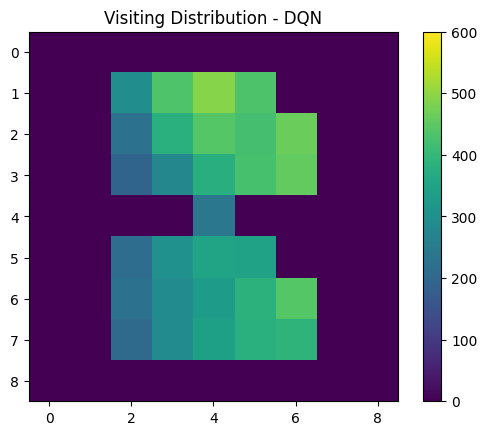
\includegraphics[width=0.70\linewidth]{Results/grid_world/visitation_distribution_dqn.png}
        \caption{DQN}
        \label{fig:visitation_distributions_dqn}
    \end{subfigure}
    \hspace*{\fill} % Adjust space between subfigures
    \begin{subfigure}{0.45\textwidth}
        \centering % Center the individual subfigure
        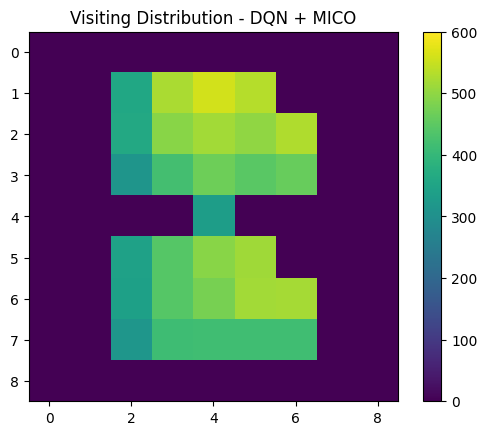
\includegraphics[width=0.70\linewidth]{Results/grid_world/visitation_distribution_dqn_mico.png}
        \caption{DQN + MICO}
        \label{fig:visitation_distributions_mico}
    \end{subfigure}
    \hspace*{\fill} % Add horizontal space to center the first two subfigures
    \vfill
    \begin{subfigure}{0.32\textwidth}
        \centering
        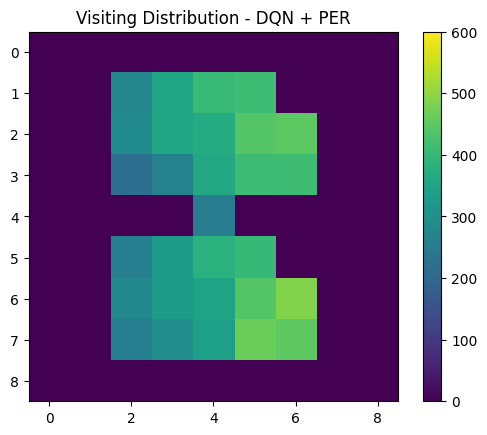
\includegraphics[width=\linewidth]{Results/grid_world/visitation_distribution_dqn_per.png}
        \caption{DQN + PER}
        \label{fig:visitation_distributions_per}
    \end{subfigure}
    \hfill
    \begin{subfigure}{0.32\textwidth}
        \centering
        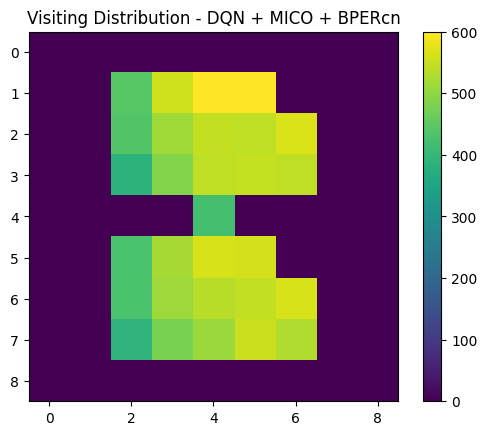
\includegraphics[width=\linewidth]{Results/grid_world/visitation_distribution_dqn_mico_bpercn.png}
        \caption{DQN + MICO + BPERcn}
        \label{fig:visitation_distributions_bpercn}
    \end{subfigure}
    \hfill
    \begin{subfigure}{0.32\textwidth}
        \centering
        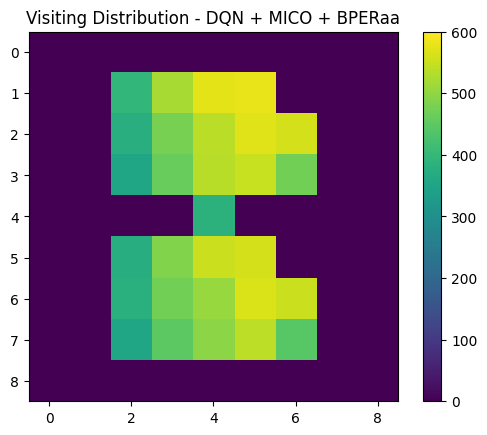
\includegraphics[width=\linewidth]{Results/grid_world/visitation_distribution_dqn_mico_bperaa.png}
        \caption{DQN + MICO + BPERaa}
        \label{fig:visitation_distributions_bperaa}
    \end{subfigure}
    \caption{Two images side-by-side}
    \label{fig:visitation_distributions}
\end{figure}


\begin{figure}
    \centering
    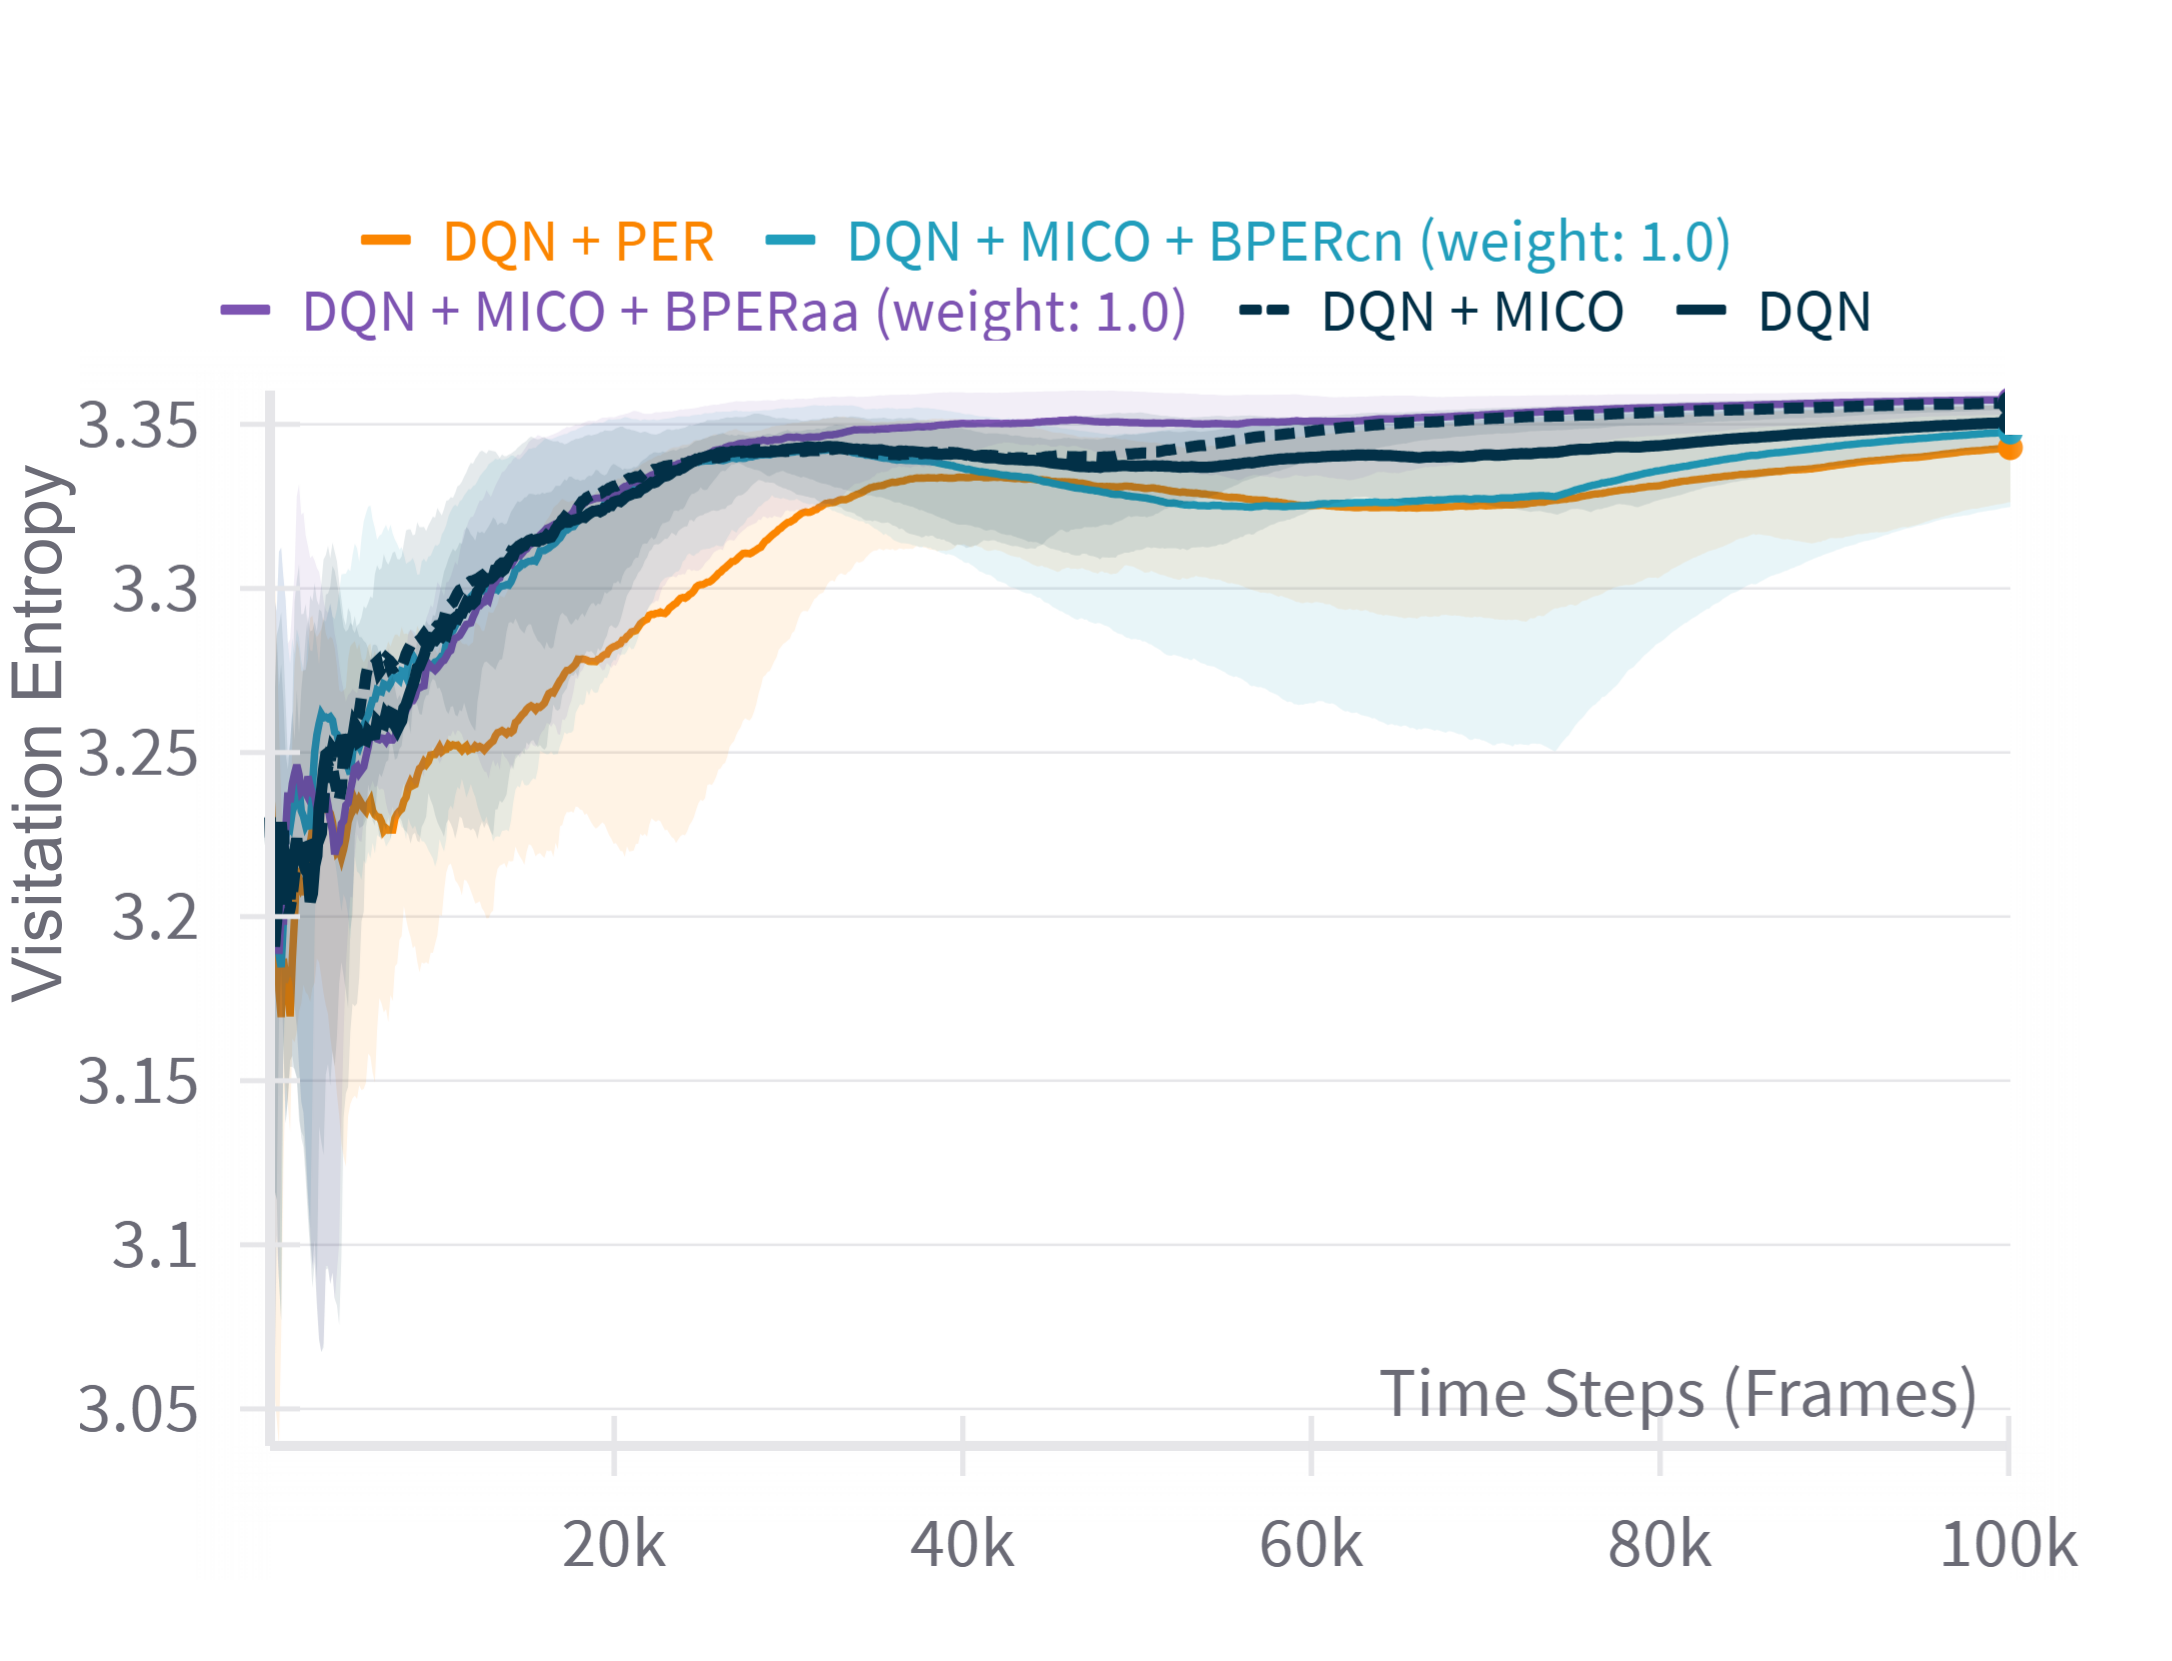
\includegraphics[width=1.\linewidth]{Results/grid_world/state_visitation_entropy.png}
    \caption{Caption}
    \label{fig:visitation_entropy}
\end{figure}


\section{General RL Performance}

After demonstrating the efficiency of the algorithm under three main problems found in the literature, we intend to explore the capabilities of the proposed method in slight complex methods. Figure \ref{fig:episode_reward_more_envs} illustrates the episode reward (100 episode window) calculated in four different environments: MountaiCar-v0, LunarLander-v1, CartPole-v1, and Acrobot-v1, average on 5 independent executions. The hyperparameter priority weight was set using the best values found\footnote{Note: There were not done an exhaustive grid search on the priority weight. Instead, the values were set following a trial and error approach, where we realized that in most of the cases when the bisimulation is no generally useful is better to set a smaller values to follow more a td-error priority}, 0.1 for Mountain Car and Cart Pole, and 1.0 for LunarLander and Acrobot. Please see Appendix \ref{} for experiments with prioritization weights 1.0 for Mountain Car and Cart Pole.

Figure \ref{fig:episode_reward_mountaincarv0} explores the episode reward on Mountain Car environment, where the bisimulation techniques, BPERcn and BPERaa, outperforms the other methods, with considerable improvements over DQN + MICO baseline. Nonetheless, it is important to note that the weight is set to 0.1, such that most of the priority will come from the td-error, implying that the bisimulation distance could does not be a useful indicator of expected learning in this scenario with binary mostly negative rewards (refer to Appendix \ref{} for results with 1.0). 

Figure \ref{fig:episode_reward_lunarlander} shows the episode reward on Lunar Lander. BPERcn and BPERaa show initially the best performance over all the methods. However, over time, the performance decreases affecting even the learning of the baseline DQN + MICO. Although, in general, the strategies outperforms the DQN and DQN + PER methods, the benefits seems to come more from the MICO learning than from the proposed strategies. 

Figure \ref{fig:episode_reward_cartpolev1} shows the episode reward on CartPole v1. In this environment, the variant PER is more consistent and outperforms the other in most of the cases. Although the BPERcn method achieves improvements over the direct baseline DQN + MICo, it does not outperforms the DQN baseline. Additionally, BPERaa outperforms both baseline DQN and DQN + MICo, but it is not better than the PER alternative. The results indicates that in this scenario the MICo learning is not producing a clear advantage over the other methods, it suggest that in this environment is complicated to discern between behavioral similar or dissimilar states due to the simple reward function and limited action space.

Figure \ref{fig:episode_reward_acrobotv1} shows the episode reward on Acrobotv1. Although the overlapping results makes difficult to analyze results, the method BPERcn and BPERaa, initially show a better performance, and eventually all will converge to a similar behavior as DQN and DQN + MICO. On the other hand, the method PER shows the worse results over time. The overlapping results makes difficult to compare the methods in such way additionally episode rewards gains were provided.


The results are quite mix, while in some escenarios is clearly to check an improvement for the proposed method in other we encounter poor results. These suggest that the effectiveness of our method is connected with the structure of the environment evaluated, specifically we hypothesis that a environement with a smoother reward function (not sparse or binary) and several actions will be optimal to prioritized behavioral disimilar staes. Specifically, because the theoretical basis leads to that tougth, it seems that the reward and transition equivalence terms in the MICO distance makes quite complex to learn behavioral states in simple scenarios were most of the states are quite similar in terms of actions and rewards. Then, by having escenarios with a more variety of actions and rewards makes the problem easier and allow us to have a better approximation of the distance and consequently of the priorities assignated to each experience. A open future work is to search complex environments were to evaluated more efficielty the capabilities of this method.


An annealing over the hyperparemeter because it seems to be more useful in the earlier steps than in the later steps.

\begin{figure}[h]
    \centering
    \begin{subfigure}{0.45\textwidth}
    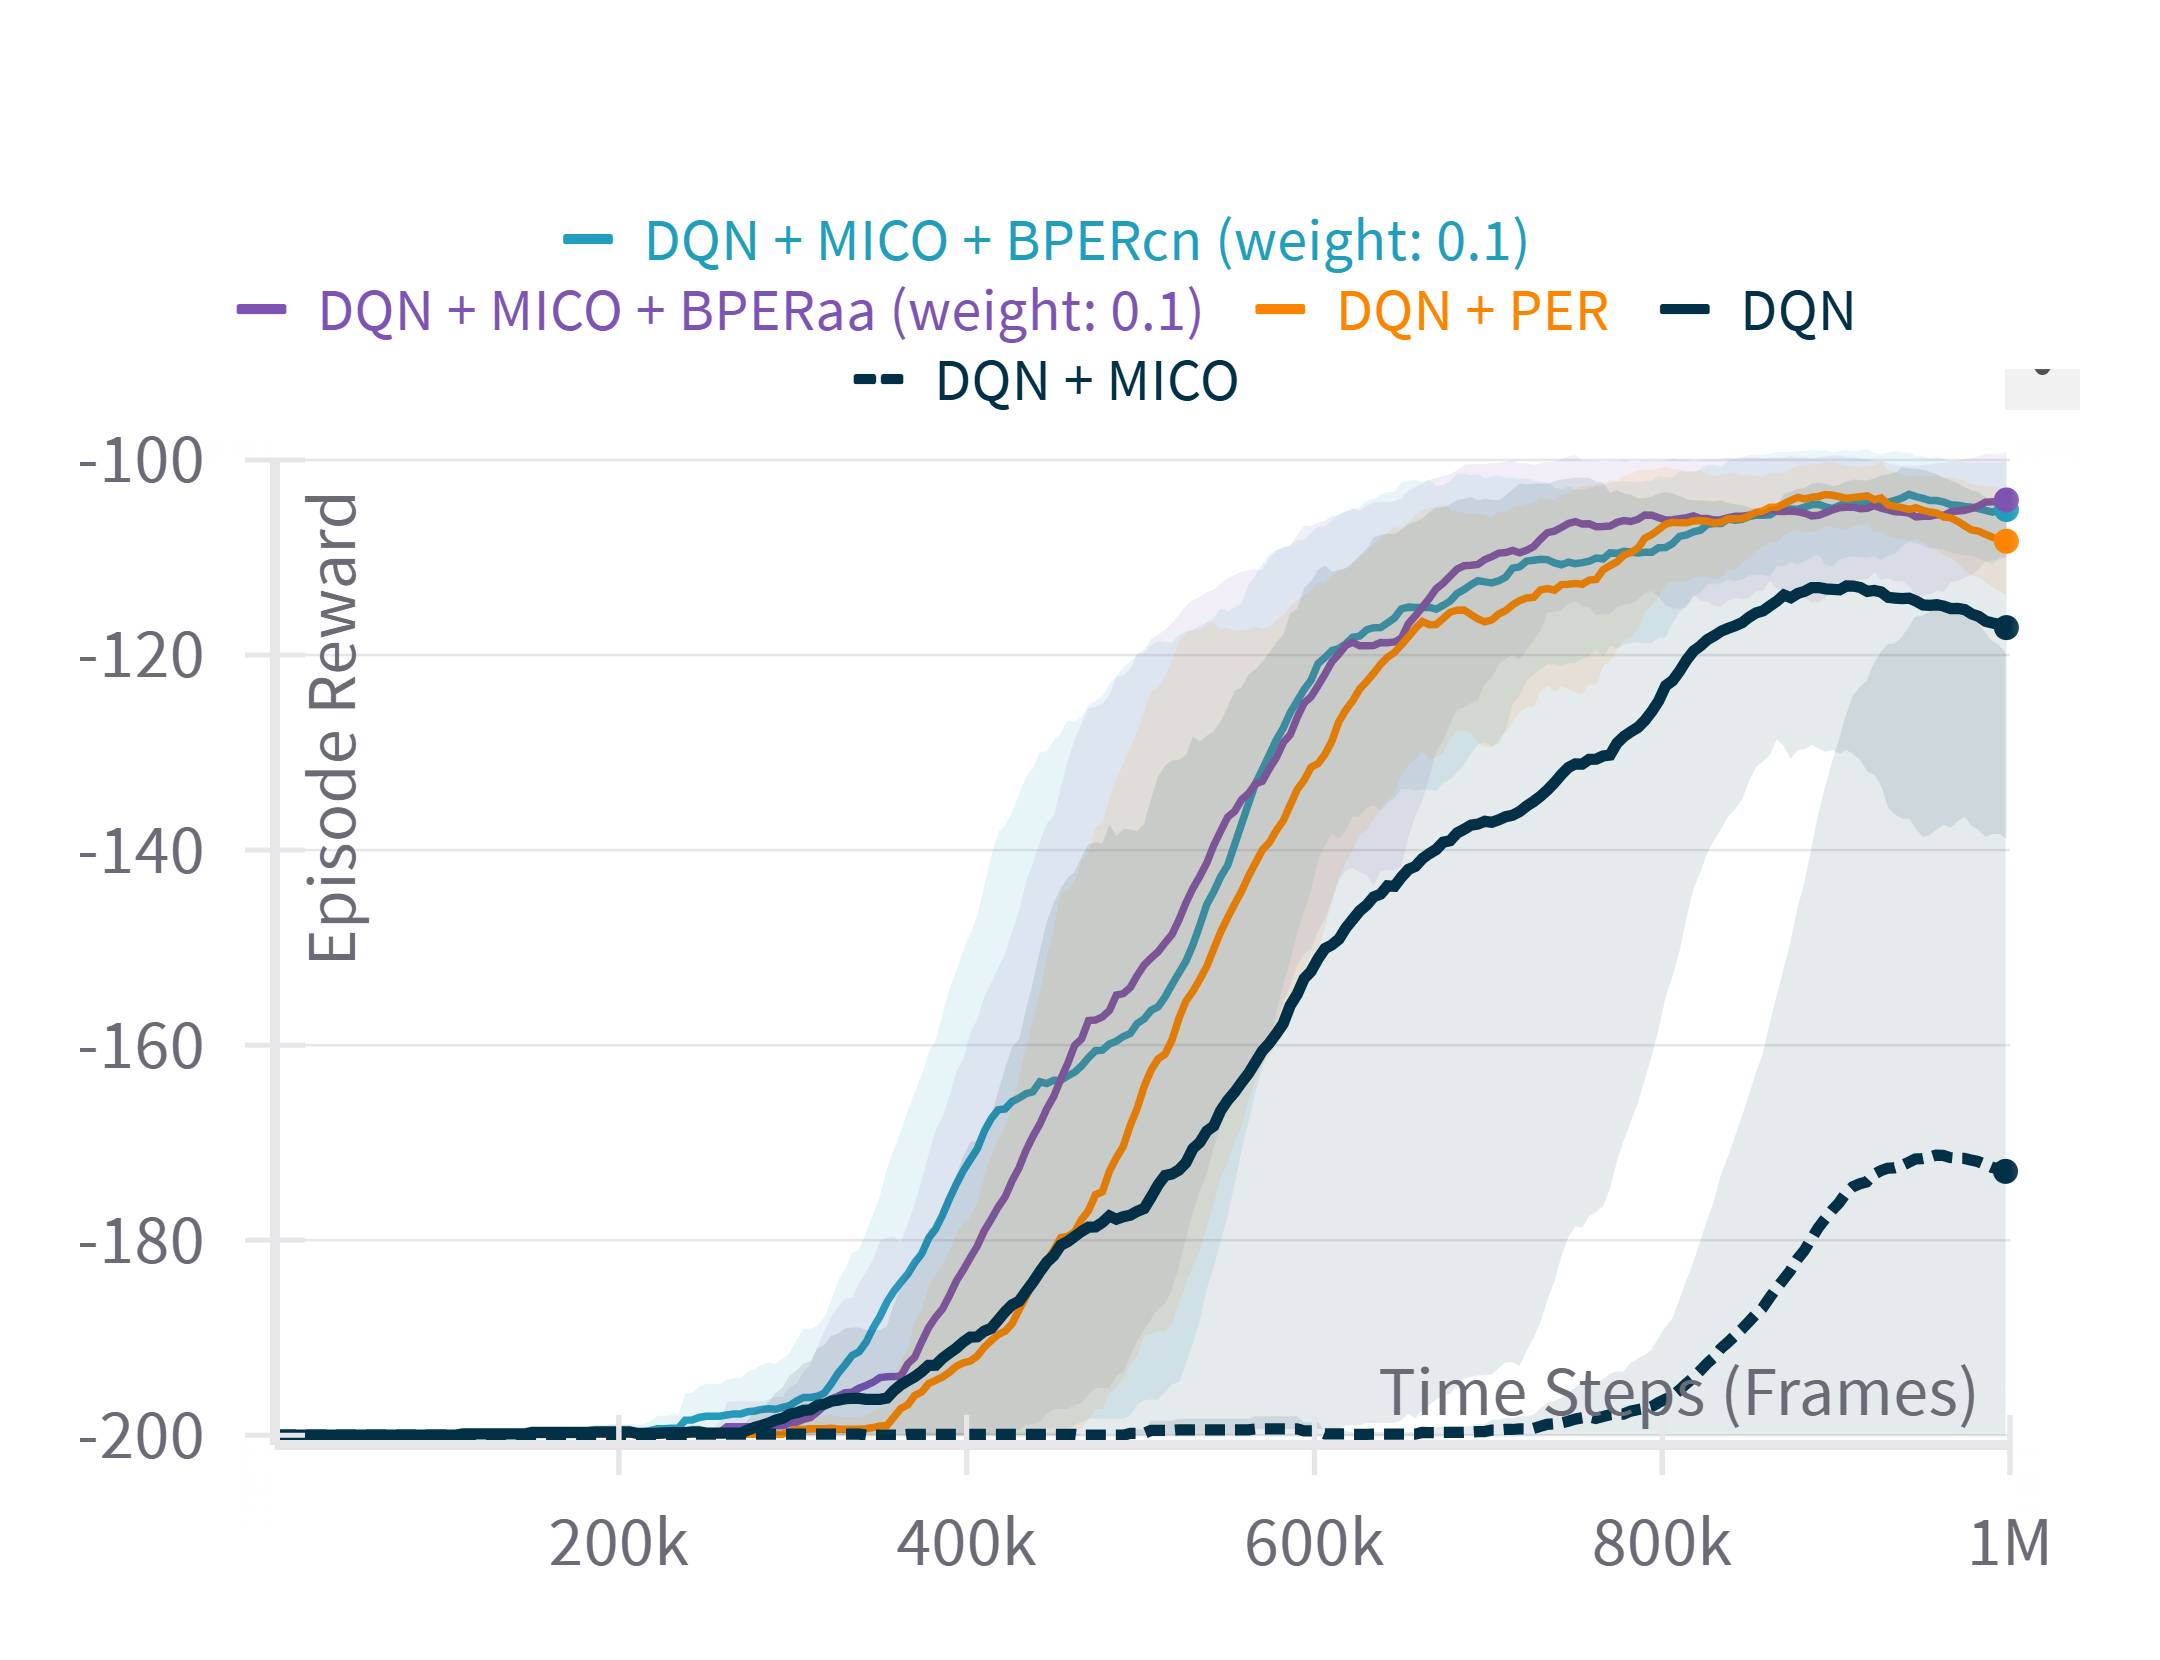
\includegraphics[width=\linewidth]{Results/general_results/episode_reward_mountaincarv0.png}
        \caption{MountainCar-v0}
        \label{fig:episode_reward_mountaincarv0}
    \end{subfigure}
    \hfill
    \begin{subfigure}{0.45\textwidth}
        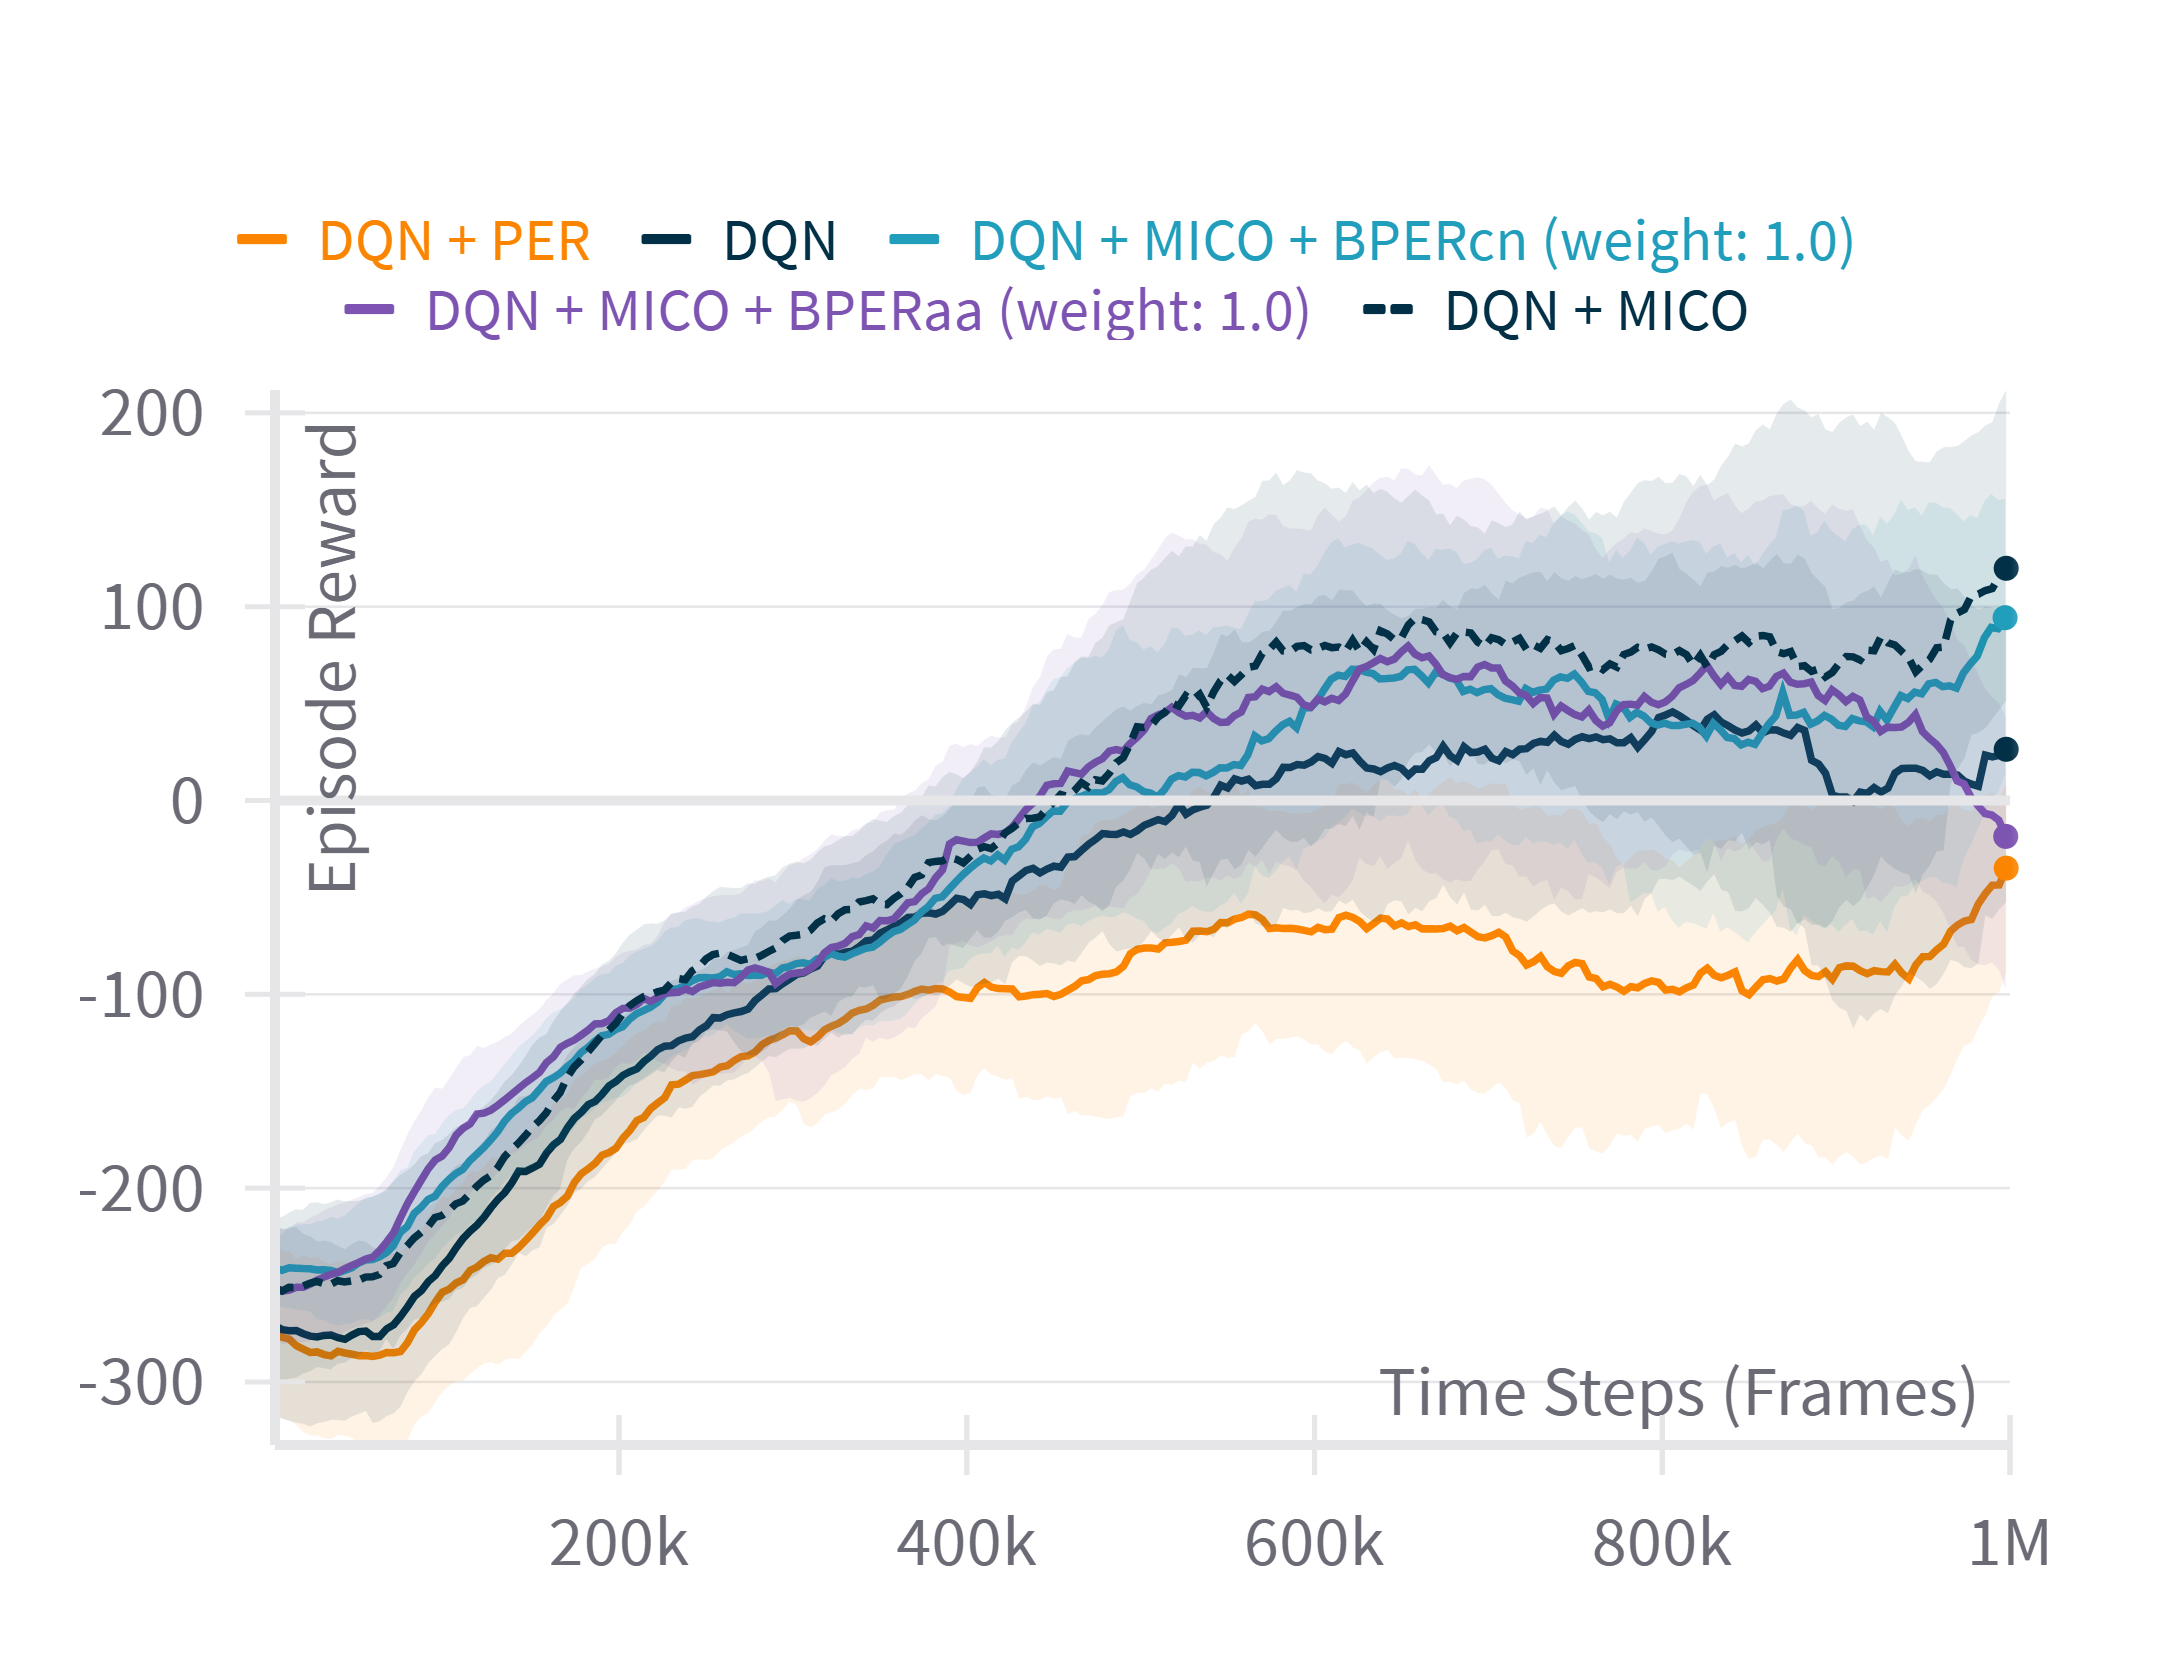
\includegraphics[width=\linewidth]{Results/general_results/episode_reward_lunarlander.png}
        \caption{LunarLander-v1}
        \label{fig:episode_reward_lunarlander}
    \end{subfigure}
    \hfill
    \begin{subfigure}{0.45\textwidth}
        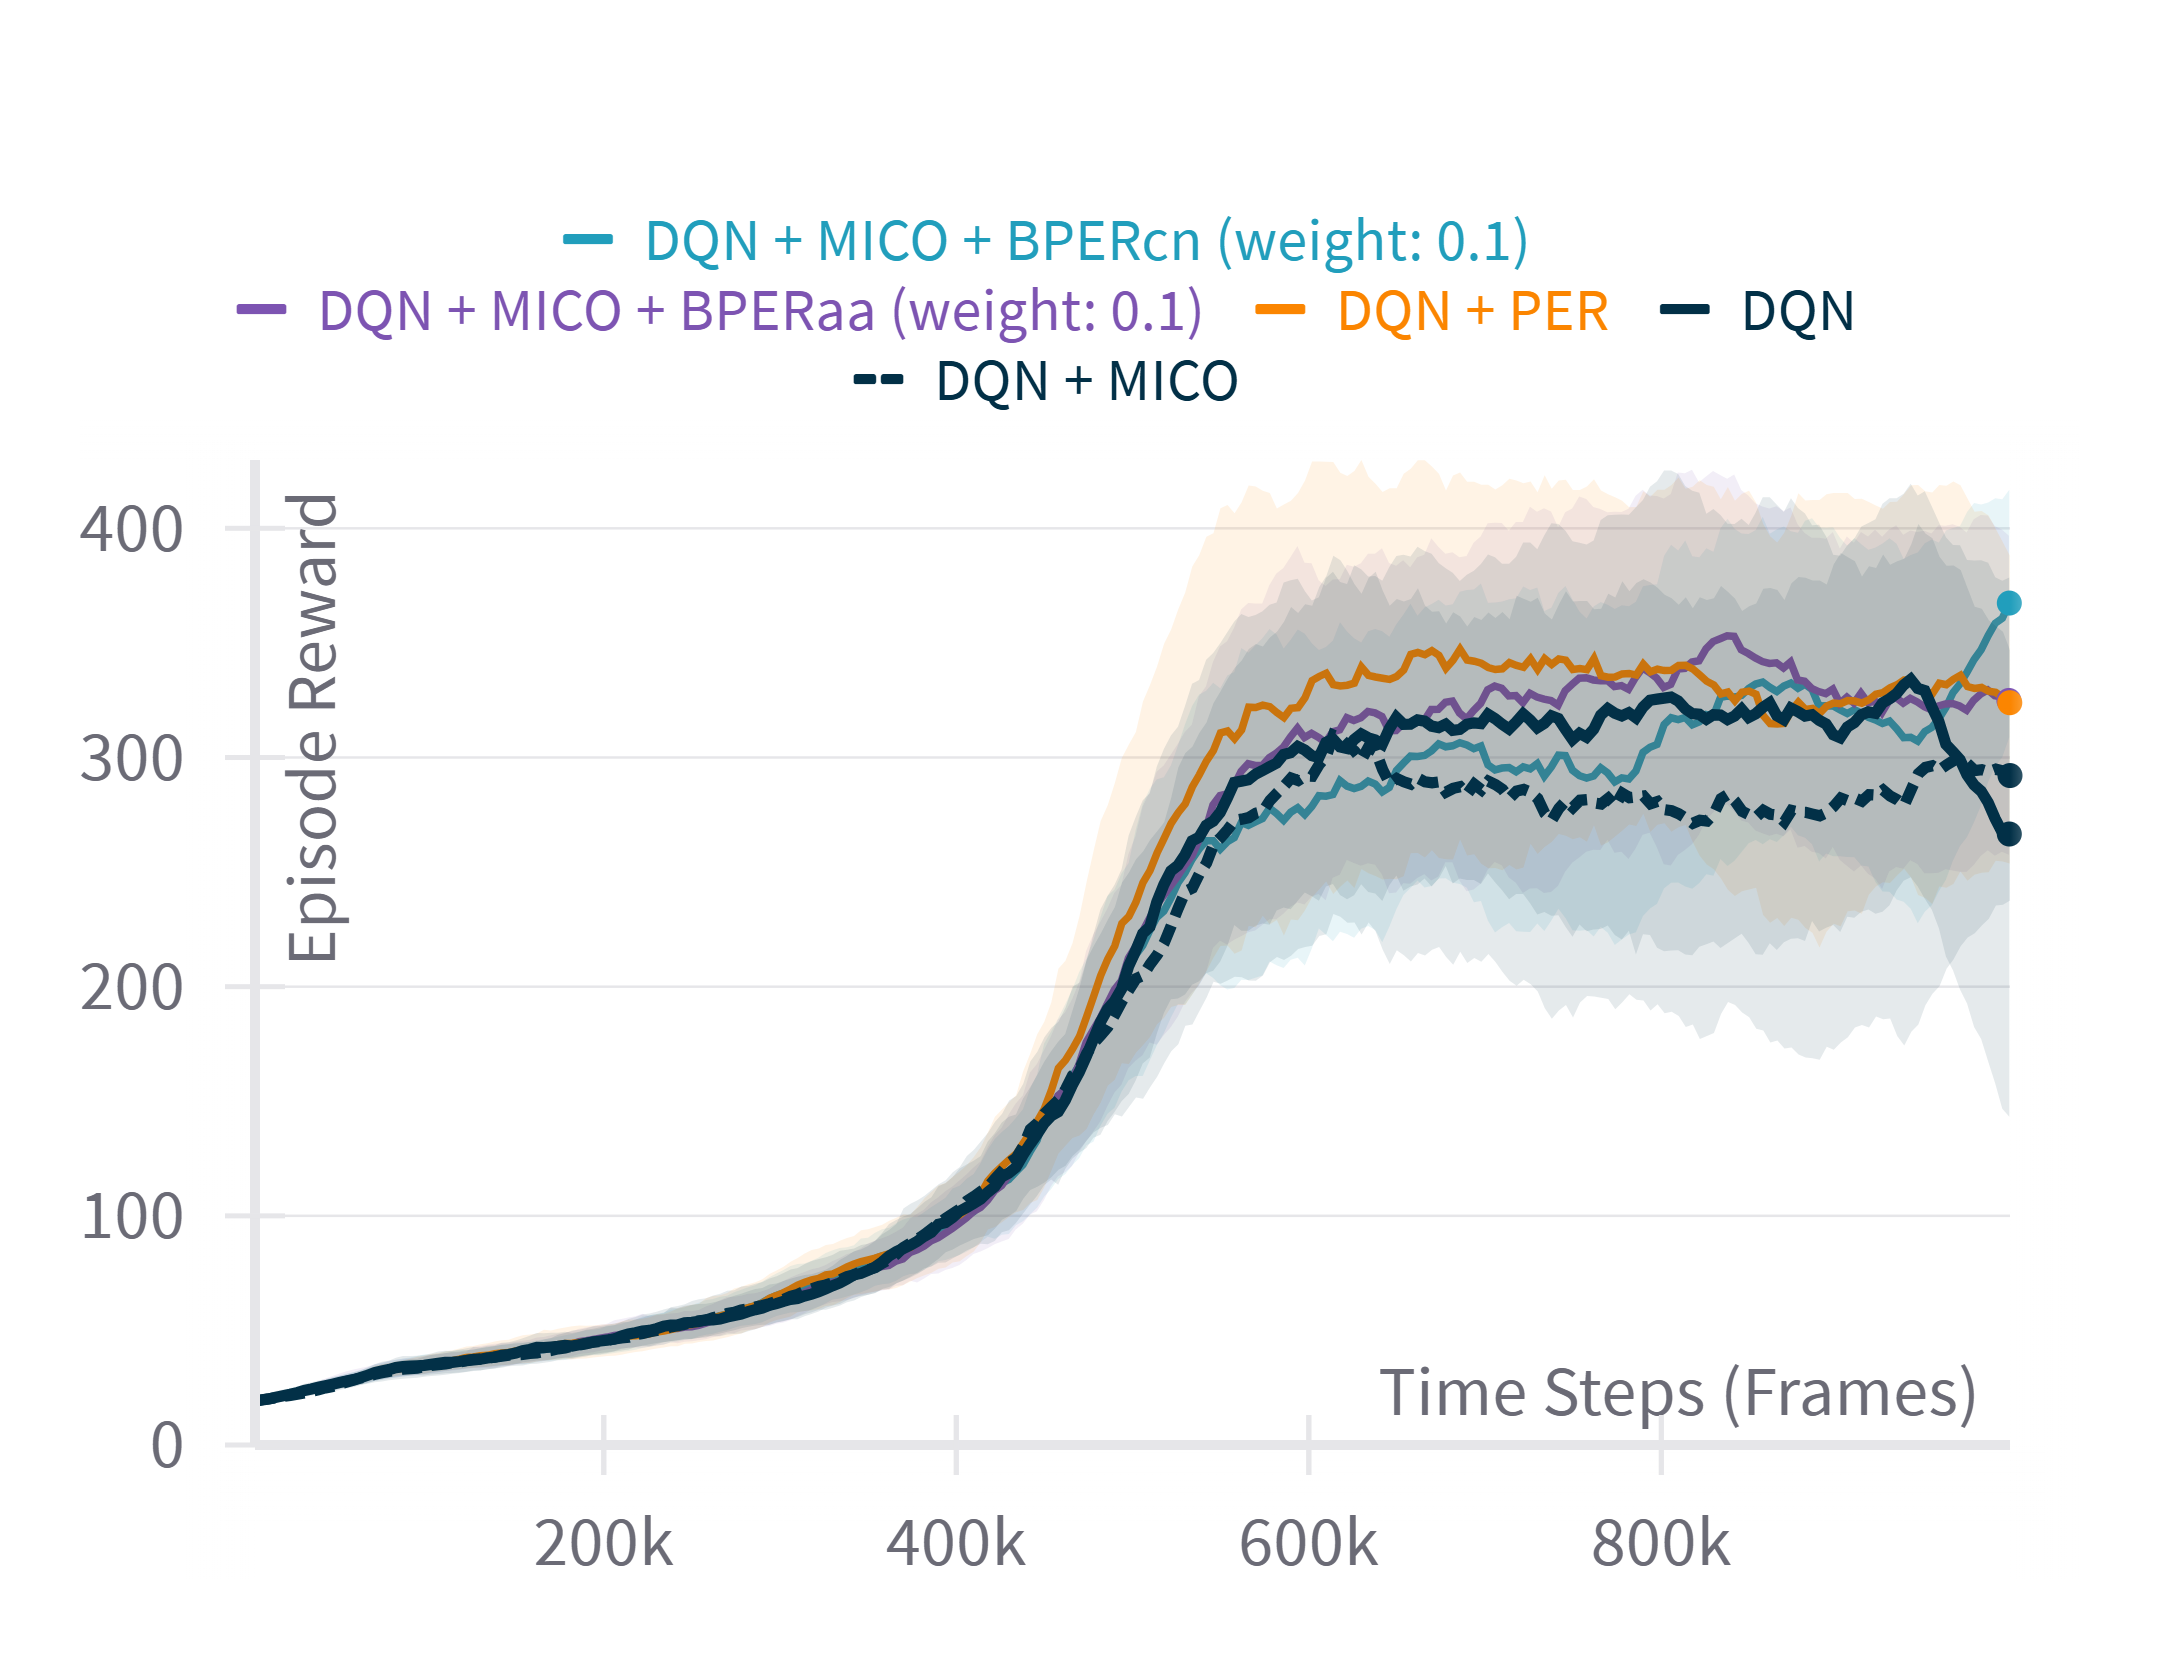
\includegraphics[width=\linewidth]{Results/general_results/episode_reward_cartpolev1.png}
        \caption{CartPole-v1}
        \label{fig:episode_reward_cartpolev1}
    \end{subfigure}
    \hfill
    \begin{subfigure}{0.45\textwidth}
        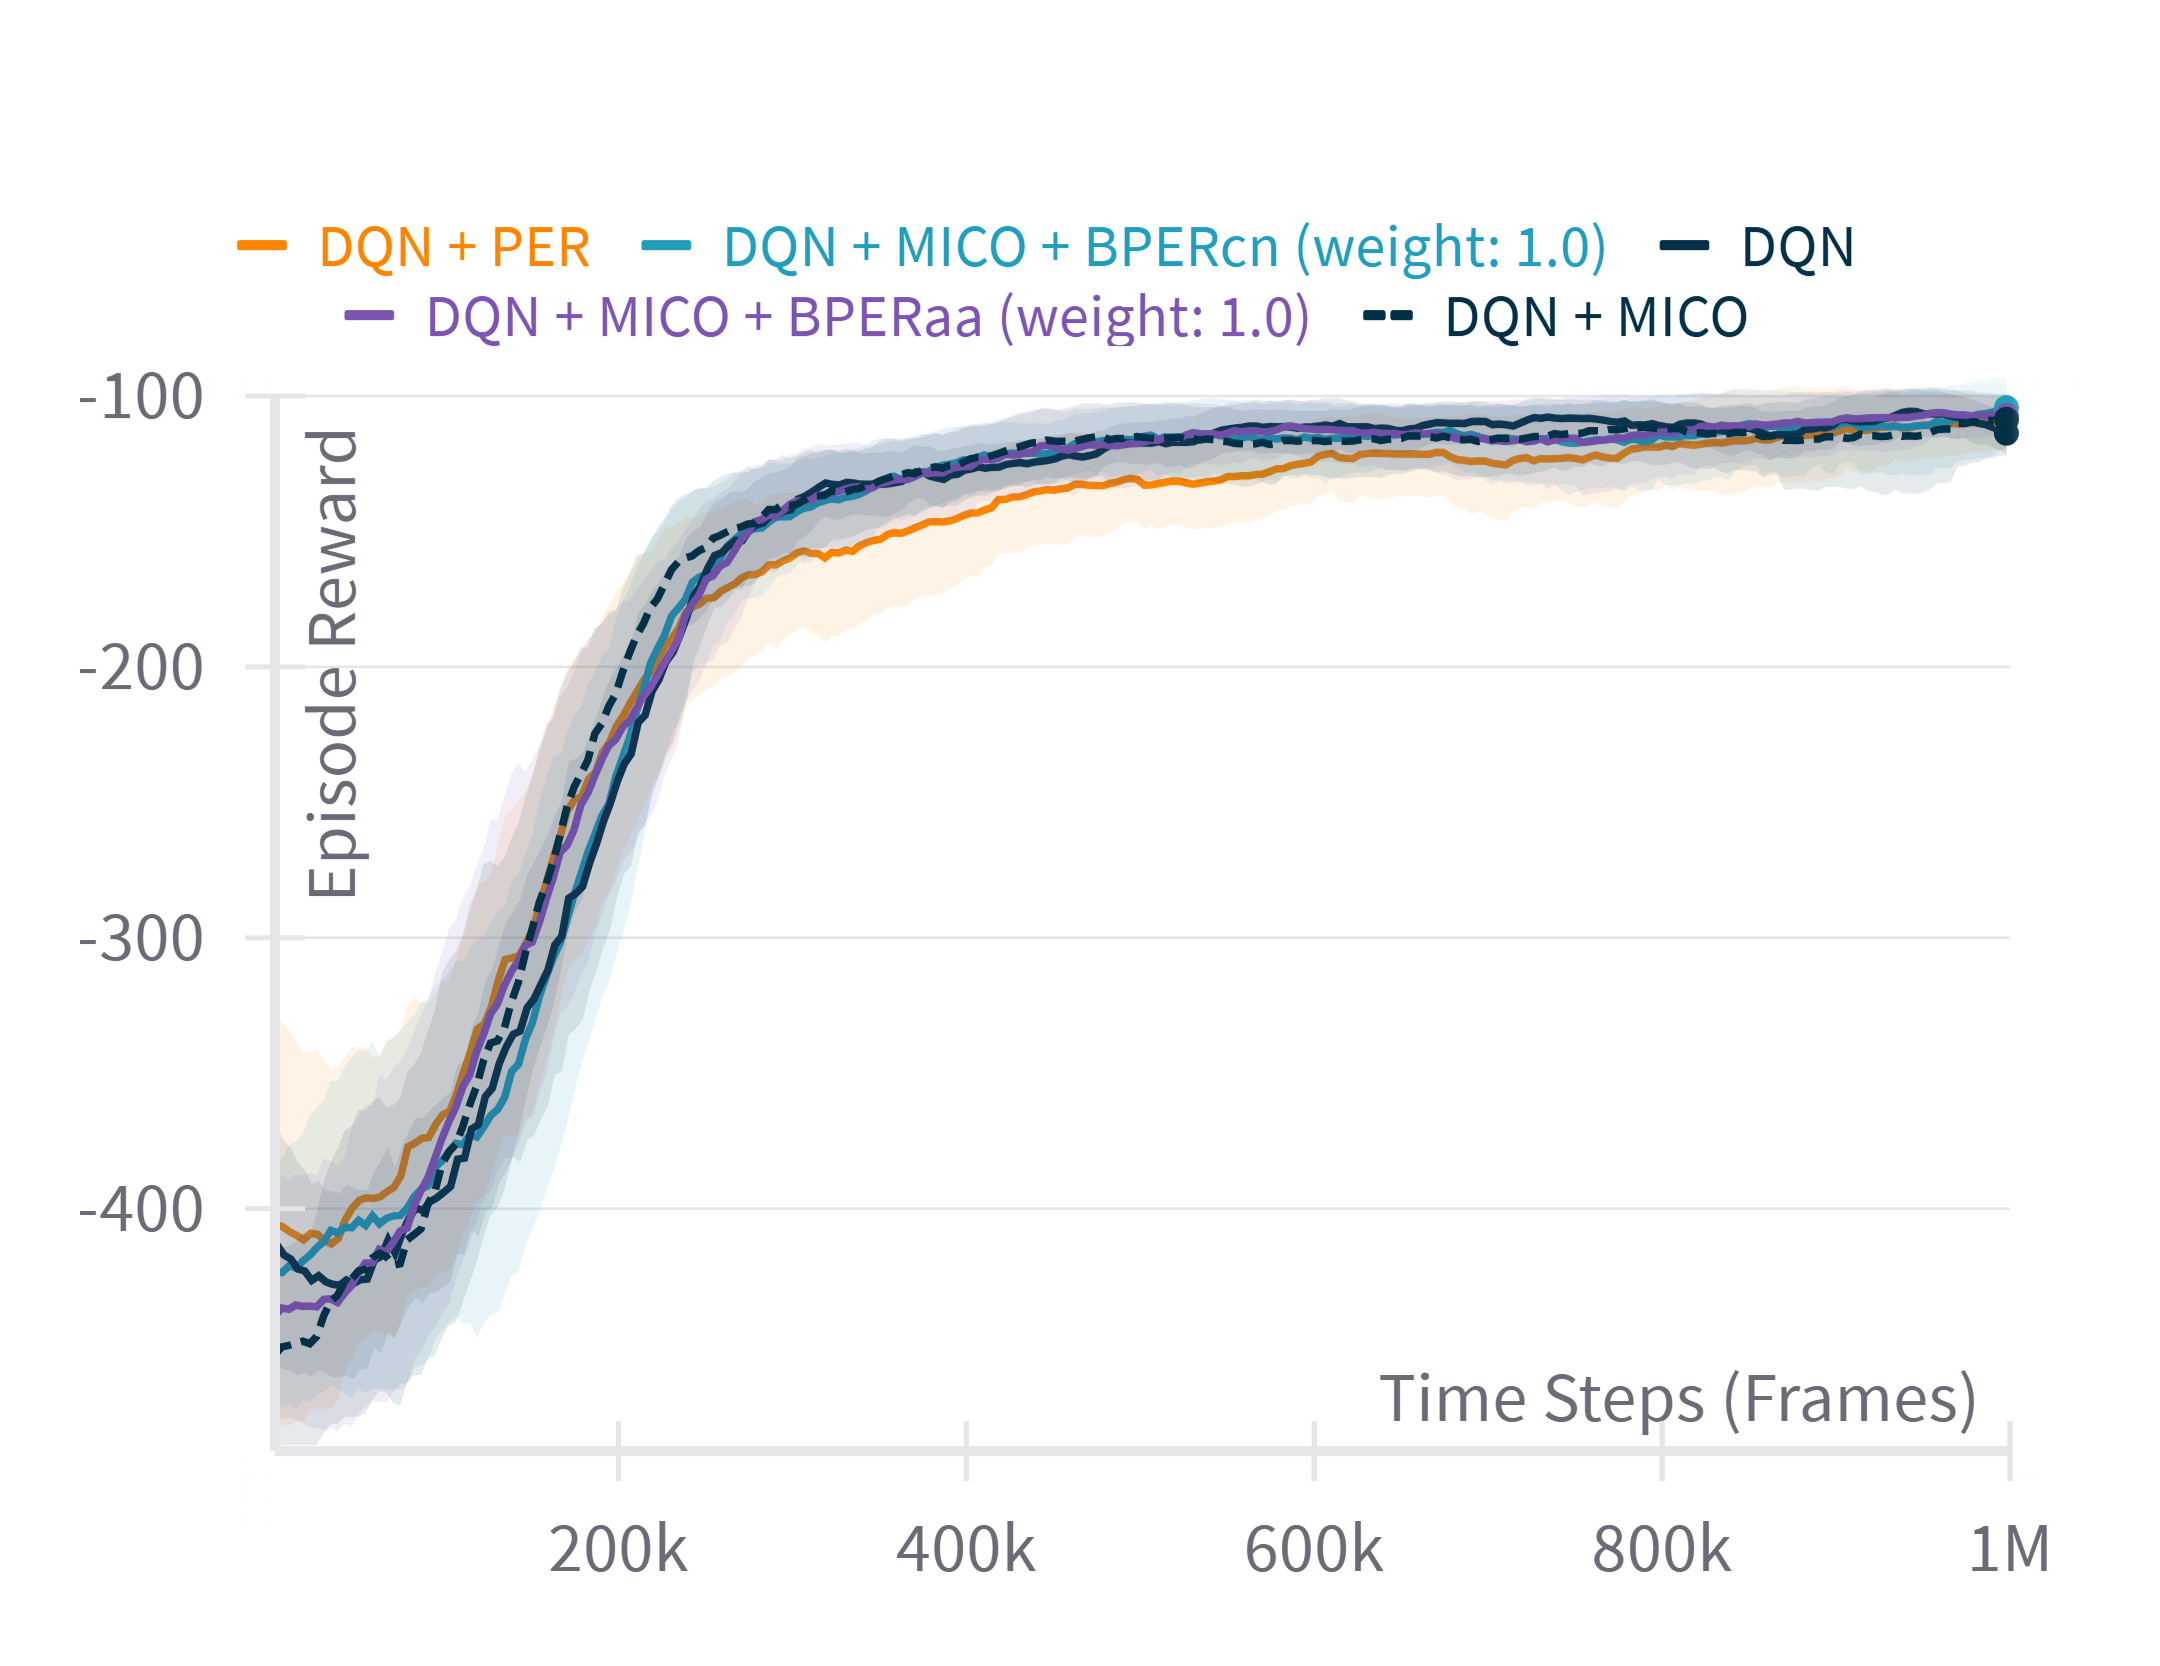
\includegraphics[width=\linewidth]{Results/general_results/episode_reward_acrobotv1.png}
        \caption{Acrobot-v1}
        \label{fig:episode_reward_acrobotv1}
    \end{subfigure}
    \caption{Two images side-by-side}
    \label{fig:episode_reward_more_envs}
\end{figure}

\begin{figure}[h]
    \centering
    \begin{subfigure}{0.45\textwidth}
    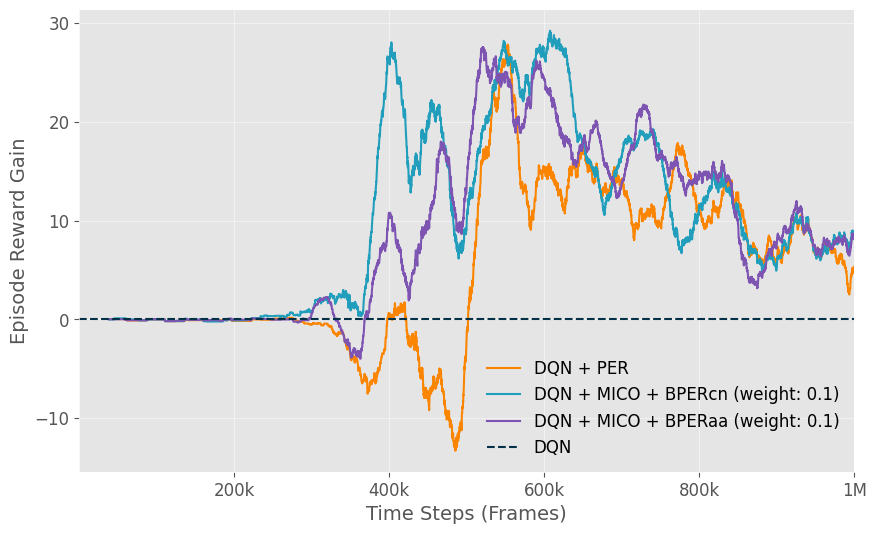
\includegraphics[width=\linewidth]{Results/general_results/mountain_car_reward_gain_vs_dqn.png}
        \caption{MountainCar-v0}
        \label{fig:on_policy_weighting}
    \end{subfigure}
    \hfill
    \begin{subfigure}{0.45\textwidth}
        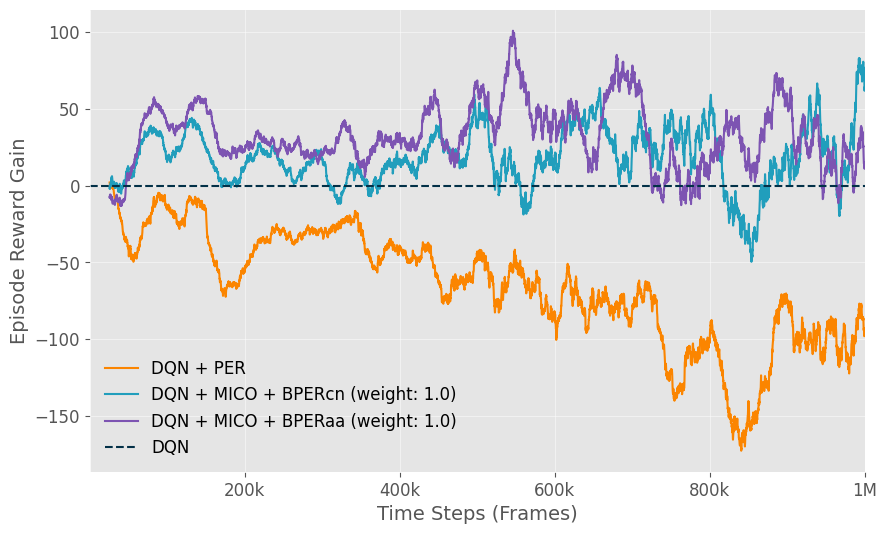
\includegraphics[width=\linewidth]{Results/general_results/lunarlander_reward_gain_vs_dqn.png}
        \caption{LunarLander-v1}
        \label{fig:uniform_weighting}
    \end{subfigure}
    \hfill
    \begin{subfigure}{0.45\textwidth}
        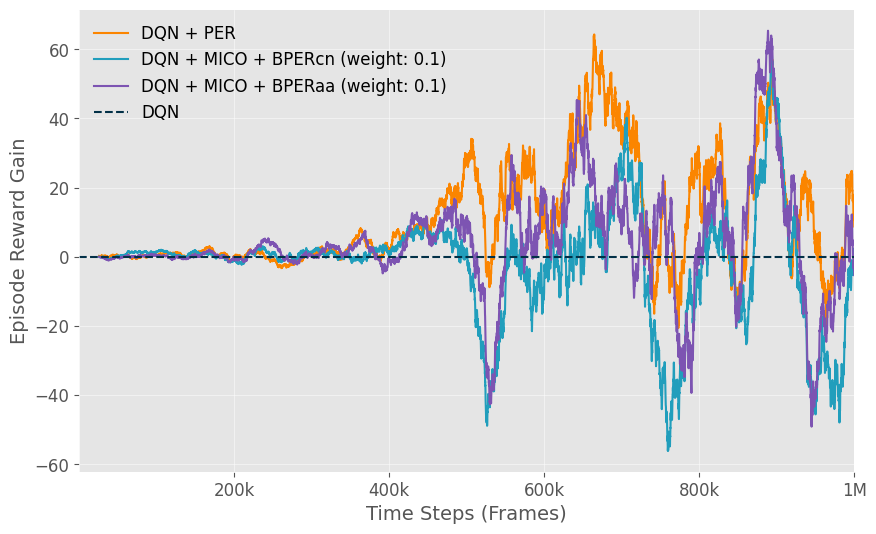
\includegraphics[width=\linewidth]{Results/general_results/cart_polev1_reward_gain_vs_dqn.png}
        \caption{CartPole-v1}
        \label{fig:uniform_weighting}
    \end{subfigure}
    \hfill
    \begin{subfigure}{0.45\textwidth}
        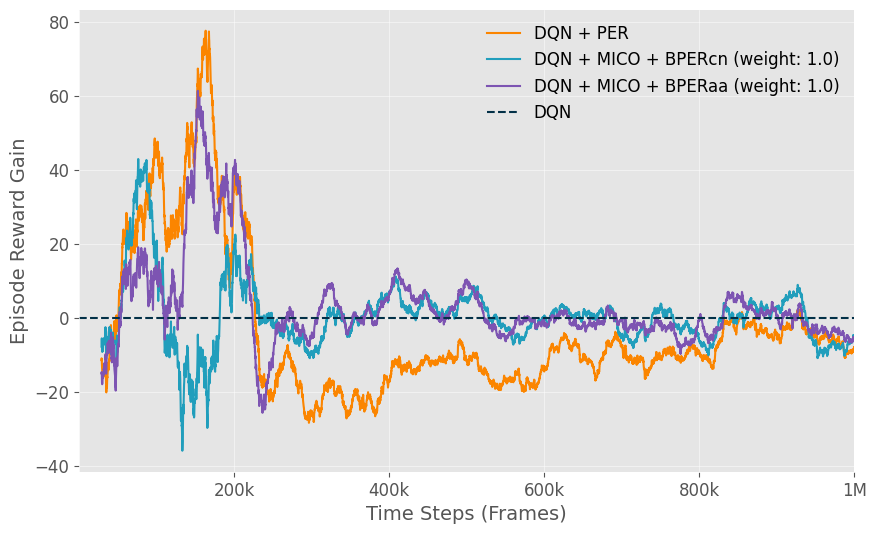
\includegraphics[width=\linewidth]{Results/general_results/acrobotv1_reward_gain_vs_dqn.png}
        \caption{Acrobot-v1}
        \label{fig:uniform_weighting}
    \end{subfigure}
    \caption{Two images side-by-side}
    \label{fig:outdated_priorities}
\end{figure}


% \begin{table}[h]
%     \centering
%     \caption{Performance Comparison of Different DQN Variants}
%     \label{tab:dqn_comparison}
%     \begin{tabular}{l >{\centering\arraybackslash}p{1.5cm} >{\centering\arraybackslash}p{1.5cm} >{\centering\arraybackslash}p{1.5cm} >{\centering\arraybackslash}p{1.5cm} >{\centering\arraybackslash}p{1.5cm} >{\centering\arraybackslash}p{1.5cm}}
%         \toprule
%                          & \multicolumn{2}{c}{\textbf{PER}}                       & \multicolumn{2}{c}{\textbf{BPERcn}}            & \multicolumn{2}{c}{\textbf{BPERaa}}             \\
%                          & {\color[HTML]{656565} \footnotesize DQN} & {\color[HTML]{656565} \footnotesize MICO} & {\color[HTML]{656565} \footnotesize DQN} & {\color[HTML]{656565} \footnotesize MICO} & {\color[HTML]{656565} \footnotesize DQN} & {\color[HTML]{656565} \footnotesize MICO} \\
%         \midrule
%         \textbf{MountainCar-v0} & $5.344 \pm 21.016$ & $39.088 \pm 39.151$   & $\mathbf{10.145} \pm \mathbf{21.471} $    & $\mathbf{43.889} \pm \mathbf{38.863}$  & $9.021 \pm 19.756$   & $42.765 \pm 39.060$     \\
%         \textbf{Cartpole-v1}    & $\mathbf{10.975} \pm \mathbf{133.140}$    & $\mathbf{24.23} \pm \mathbf{135.122}$   & $-2.100 \pm 134.322$   & $11.648 \pm 129.970$  & $3.790 \pm 134.959$    & $17.539 \pm 134.593$     \\
%         \textbf{Acrobot-v1}     & $-3.279 \pm 79.455$  & $-6.878 \pm 74.916$   & $0.250 \pm 78.057$    & $-3.350 \pm 73.122$  & $\mathbf{2.915} \pm \mathbf{75.618}$    & $\mathbf{-0.685} \pm \mathbf{70.853}$     \\
%         \textbf{LunarLander-v1} & $-65.620 \pm 175.613$    & $-107.075 \pm 183.781$   & $18.800 \pm 191.309$    & $-22.654 \pm 194.957$  & $\mathbf{32.125} \pm \mathbf{185.015}$    & $\mathbf{-9.330} \pm \mathbf{191.315}$   \\
%         \bottomrule
%     \end{tabular}
% \end{table}

\begin{table}[h]
    \hspace*{-1cm}
    \setlength{\tabcolsep}{2.5pt}
    \centering
    \begin{tabular}{llcccc}
        \toprule
        & \textbf{Baseline} & \textbf{MountainCar-v0} & \textbf{Cartpole-v1} & \textbf{Acrobot-v1} & \textbf{LunarLander-v1} \\
        \midrule
        {\footnotesize\textbf{PER}} & {\footnotesize\textbf{DQN}} & $5.344 \pm 21.016$ & $\mathbf{10.975} \pm \mathbf{133.140}$ & $-3.279 \pm 79.455$ & $-65.620 \pm 175.613$ \\
         & {\footnotesize\textbf{MICO}} & $39.088 \pm 39.151$ & $\mathbf{24.23} \pm \mathbf{135.122}$ & $-6.878 \pm 74.916$ & $-107.075 \pm 183.781$ \\
        {\footnotesize\textbf{BPERcn}} & {\footnotesize\textbf{DQN}} & $\mathbf{10.145} \pm \mathbf{21.471}$ & $-2.100 \pm 134.322$ & $0.250 \pm 78.057$ & $18.800 \pm 191.309$ \\
        & {\footnotesize\textbf{MICO}} & $\mathbf{43.889} \pm \mathbf{38.863}$ & $11.648 \pm 129.970$ & $-3.350 \pm 73.122$ & $-22.654 \pm 194.957$ \\
        {\footnotesize\textbf{BPERaa}} & {\footnotesize\textbf{DQN}} & $9.021 \pm 19.756$ & $3.790 \pm 134.959$ & $\mathbf{2.915} \pm \mathbf{75.618}$ & $\mathbf{32.125} \pm \mathbf{185.015}$ \\
        & {\footnotesize\textbf{MICO}} & $42.765 \pm 39.060$ & $17.539 \pm 134.593$ & $\mathbf{-0.685} \pm \mathbf{70.853}$ & $\mathbf{-9.330} \pm \mathbf{191.315}$ \\
        \bottomrule
    \end{tabular}
    \caption{Performance Comparison of Different DQN Variants}
    \label{tab:dqn_comparison_transposed}
\end{table}

\begin{figure}[h]
    \centering
    \begin{subfigure}{0.45\textwidth}
    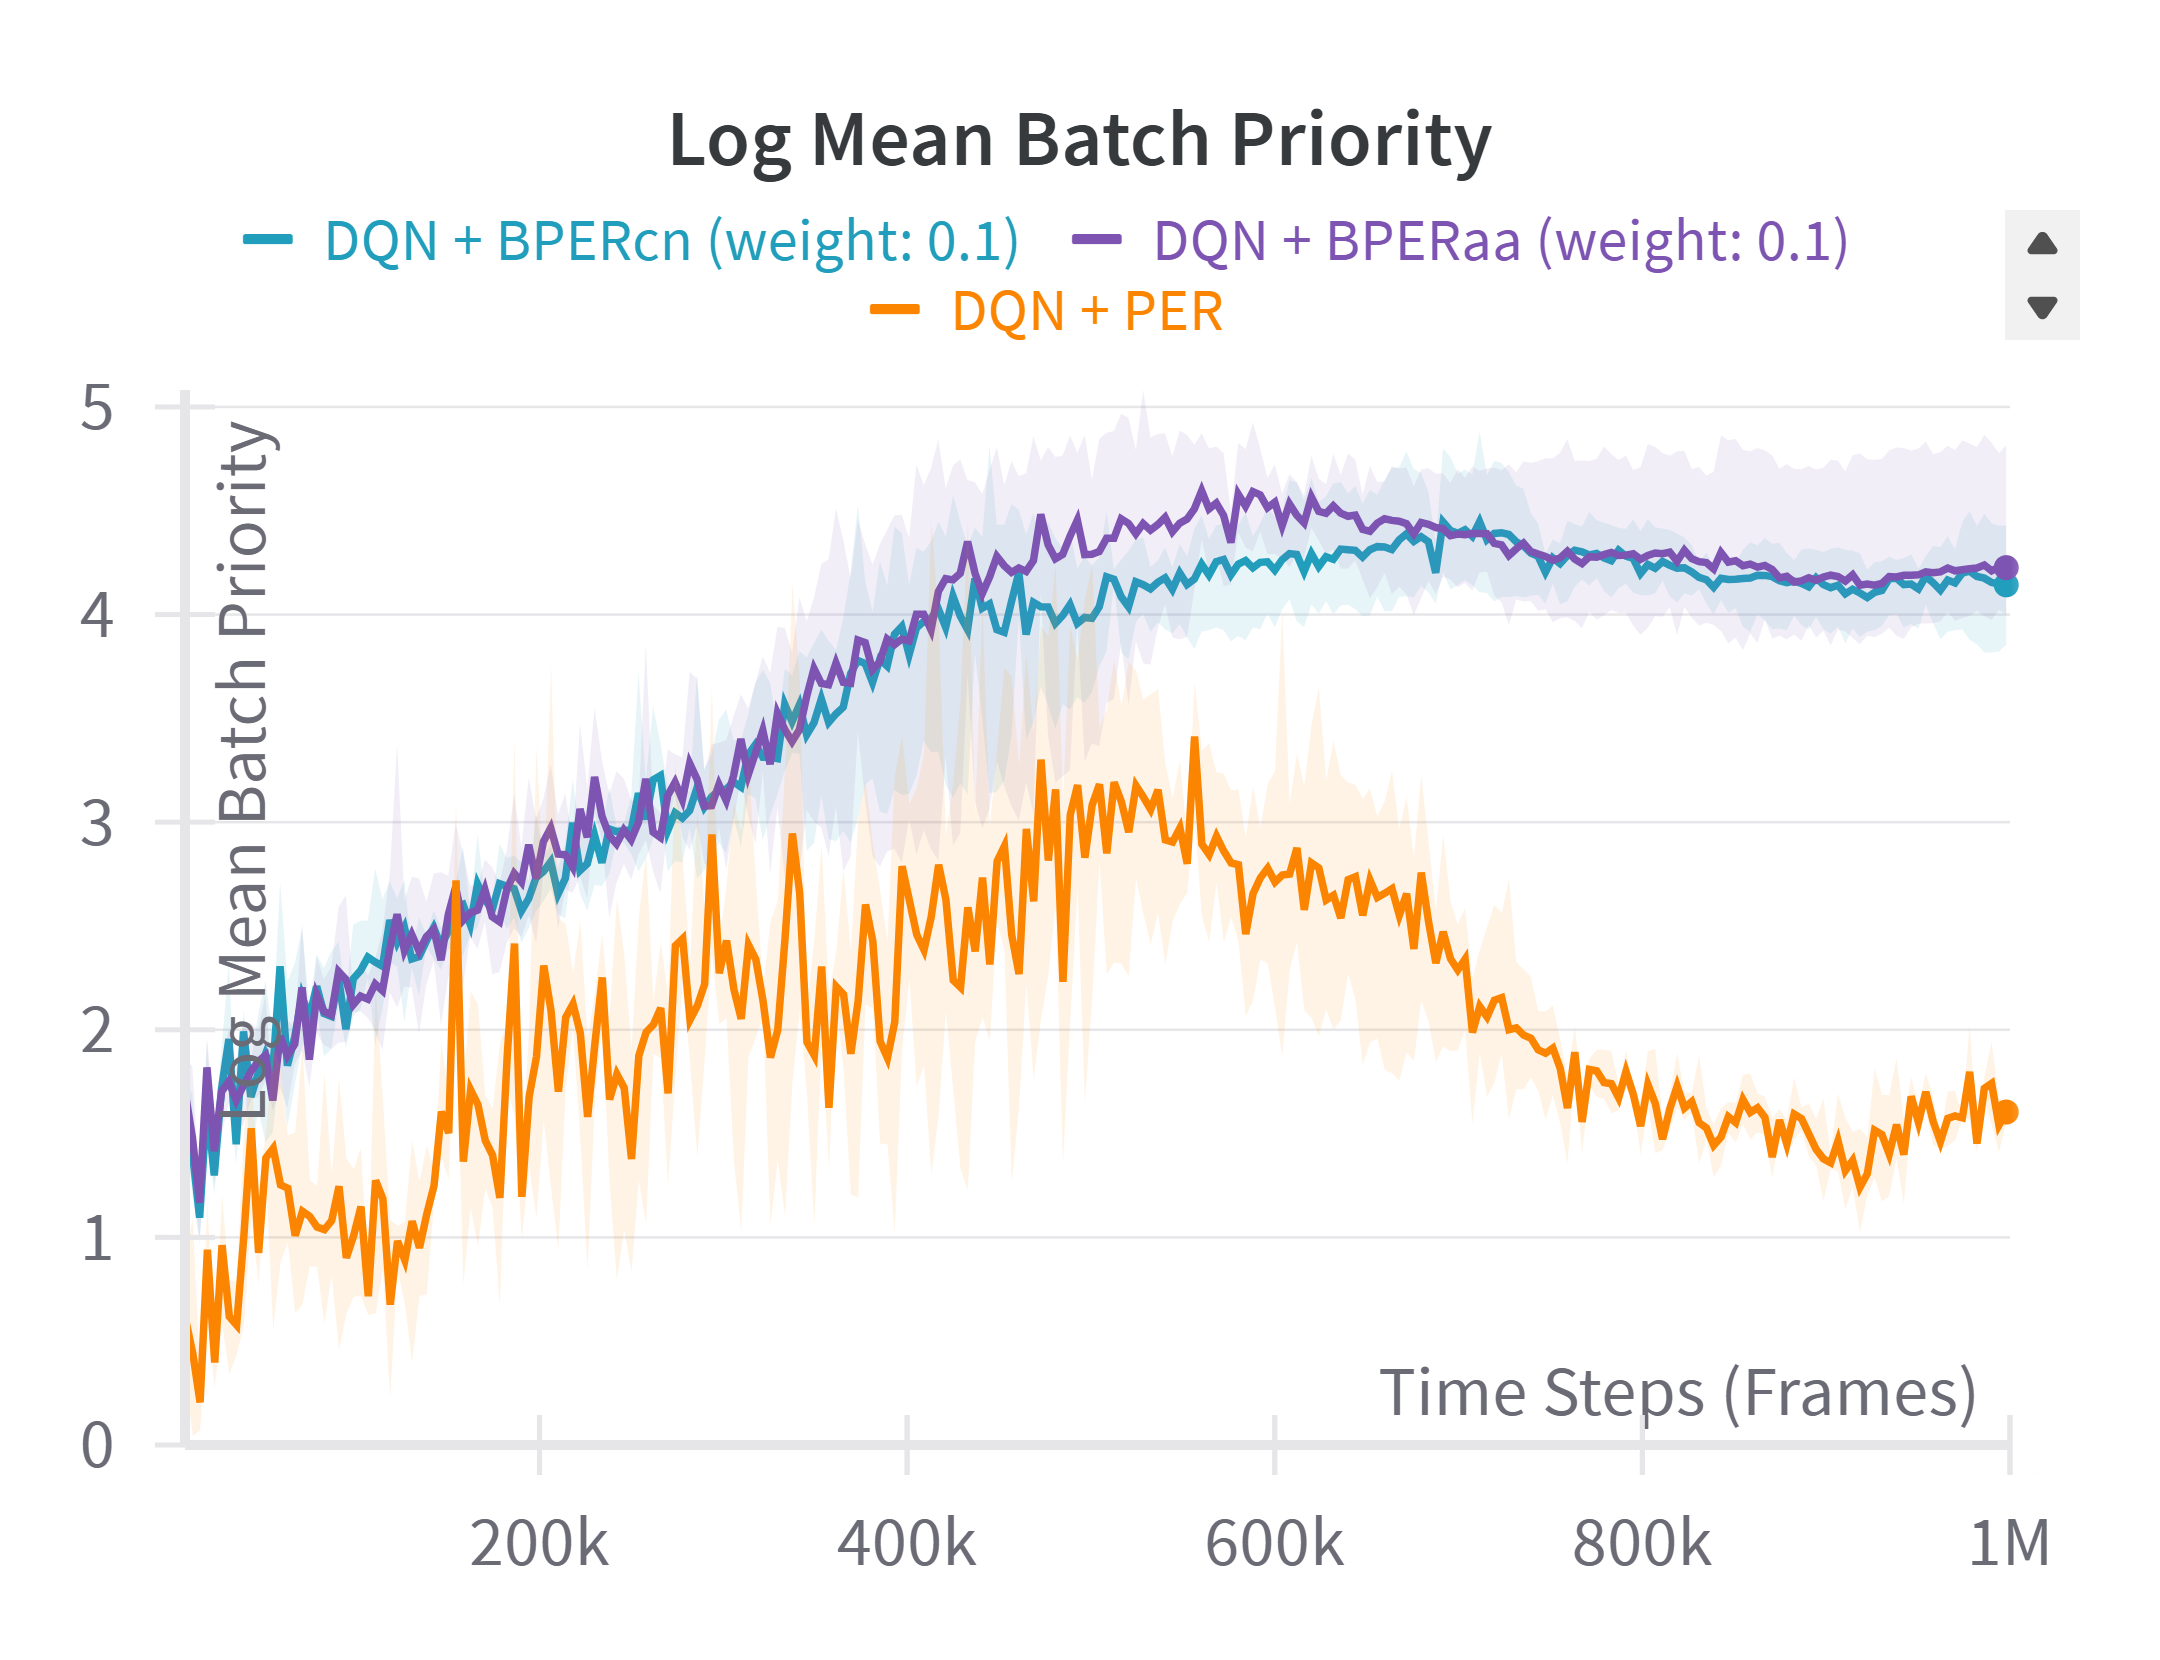
\includegraphics[width=\linewidth]{Results/general_results/log_mean_batch_priority_mountain_car.png}
        \caption{MountainCar-v0}
        \label{fig:on_policy_weighting}
    \end{subfigure}
    \hfill
    \begin{subfigure}{0.45\textwidth}
        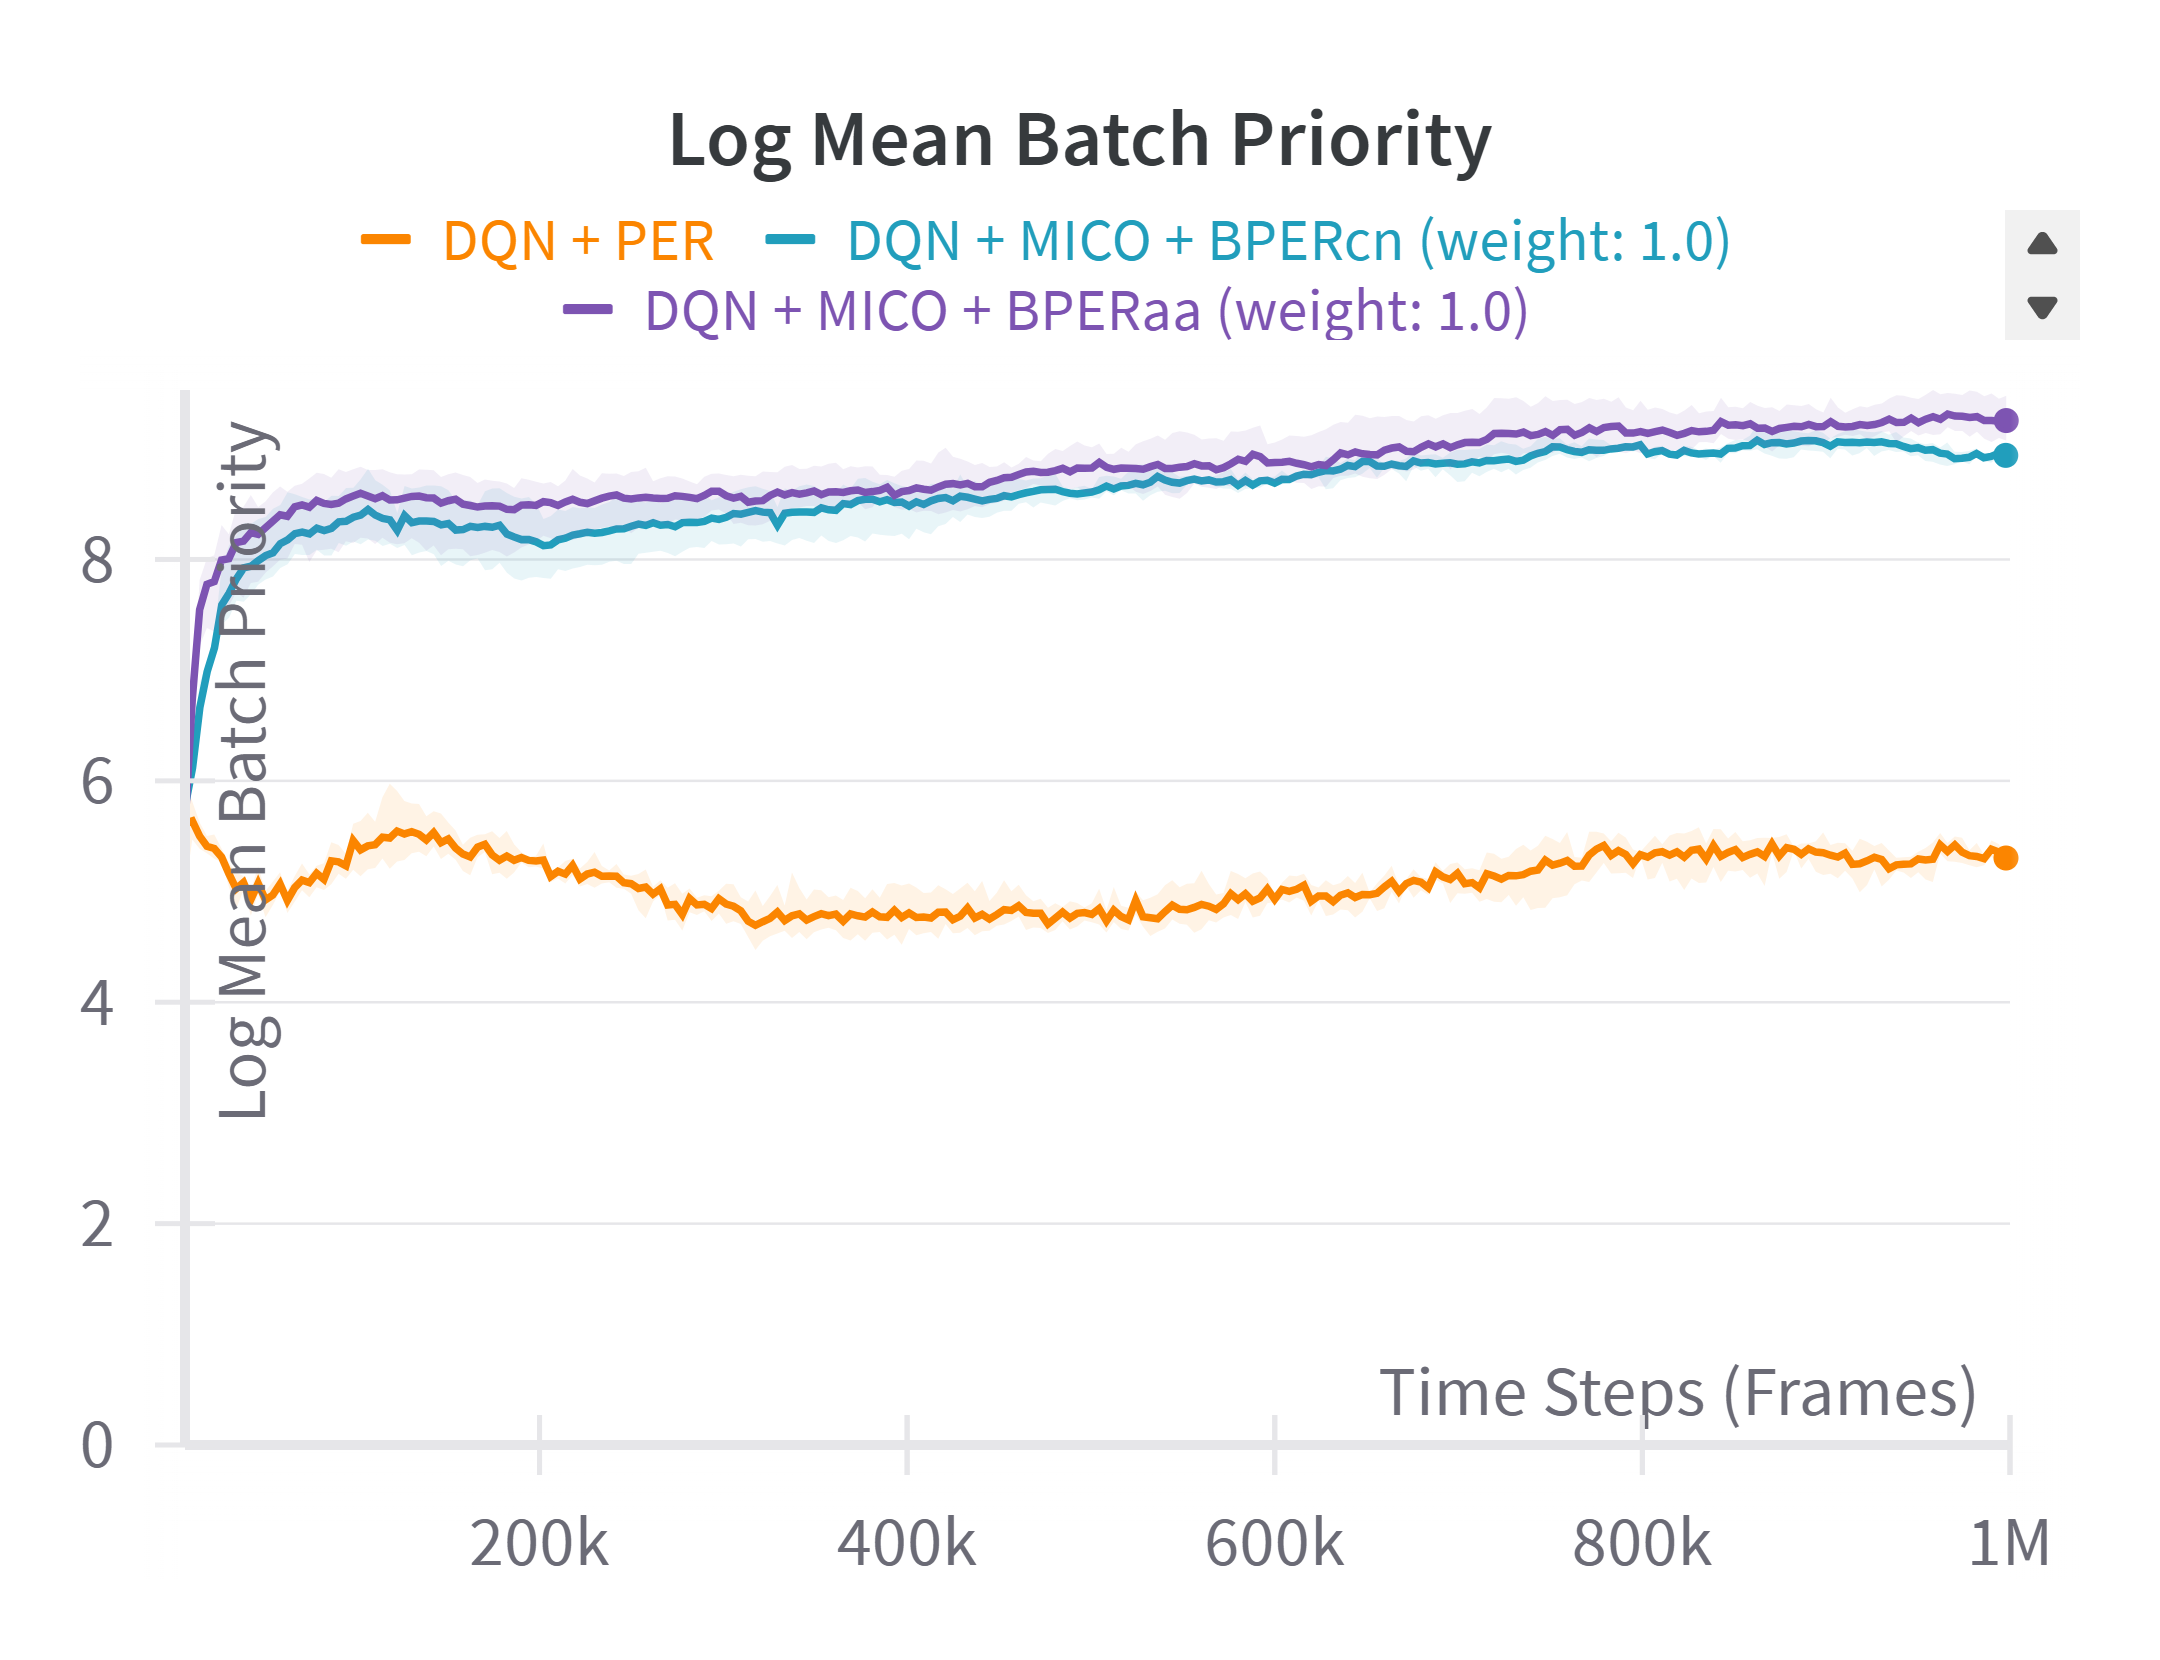
\includegraphics[width=\linewidth]{Results/general_results/log_mean_batch_priority_lunarlander.png}
        \caption{LunarLander-v1}
        \label{fig:uniform_weighting}
    \end{subfigure}
    \hfill
    \begin{subfigure}{0.45\textwidth}
        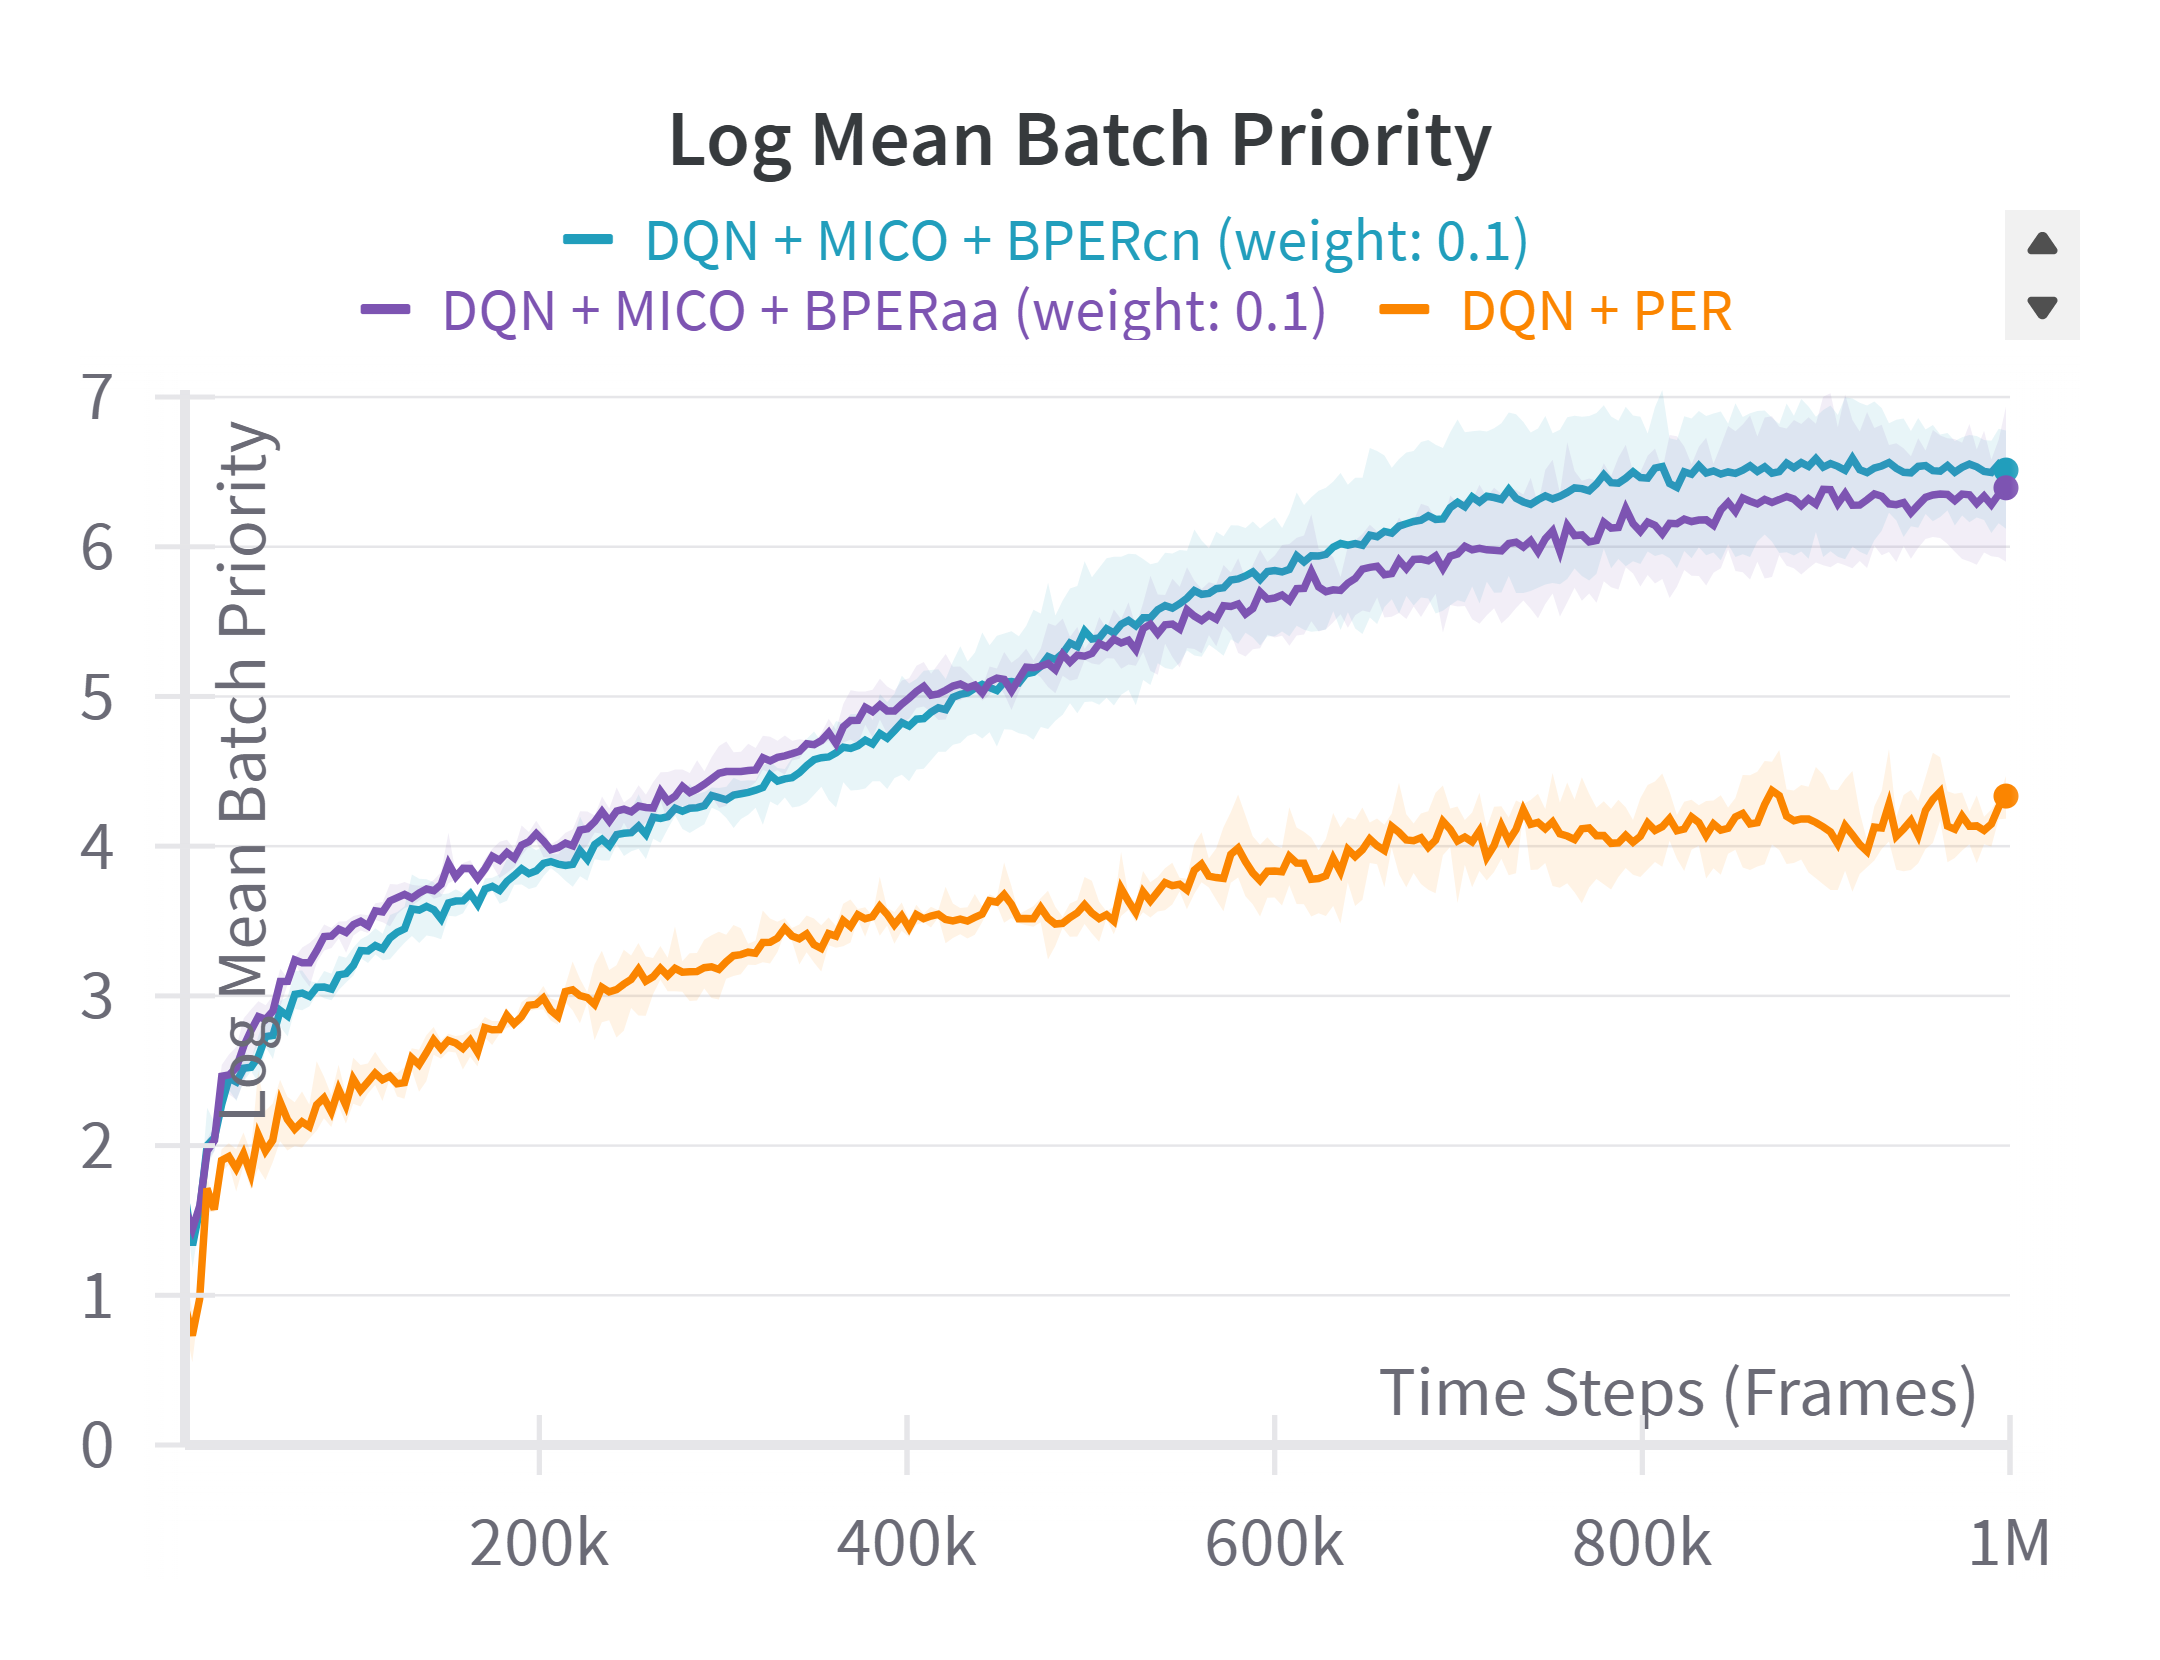
\includegraphics[width=\linewidth]{Results/general_results/log_mean_batch_priority_cartpolev1.png}
        \caption{CartPole-v1}
        \label{fig:uniform_weighting}
    \end{subfigure}
    \hfill
    \begin{subfigure}{0.45\textwidth}
        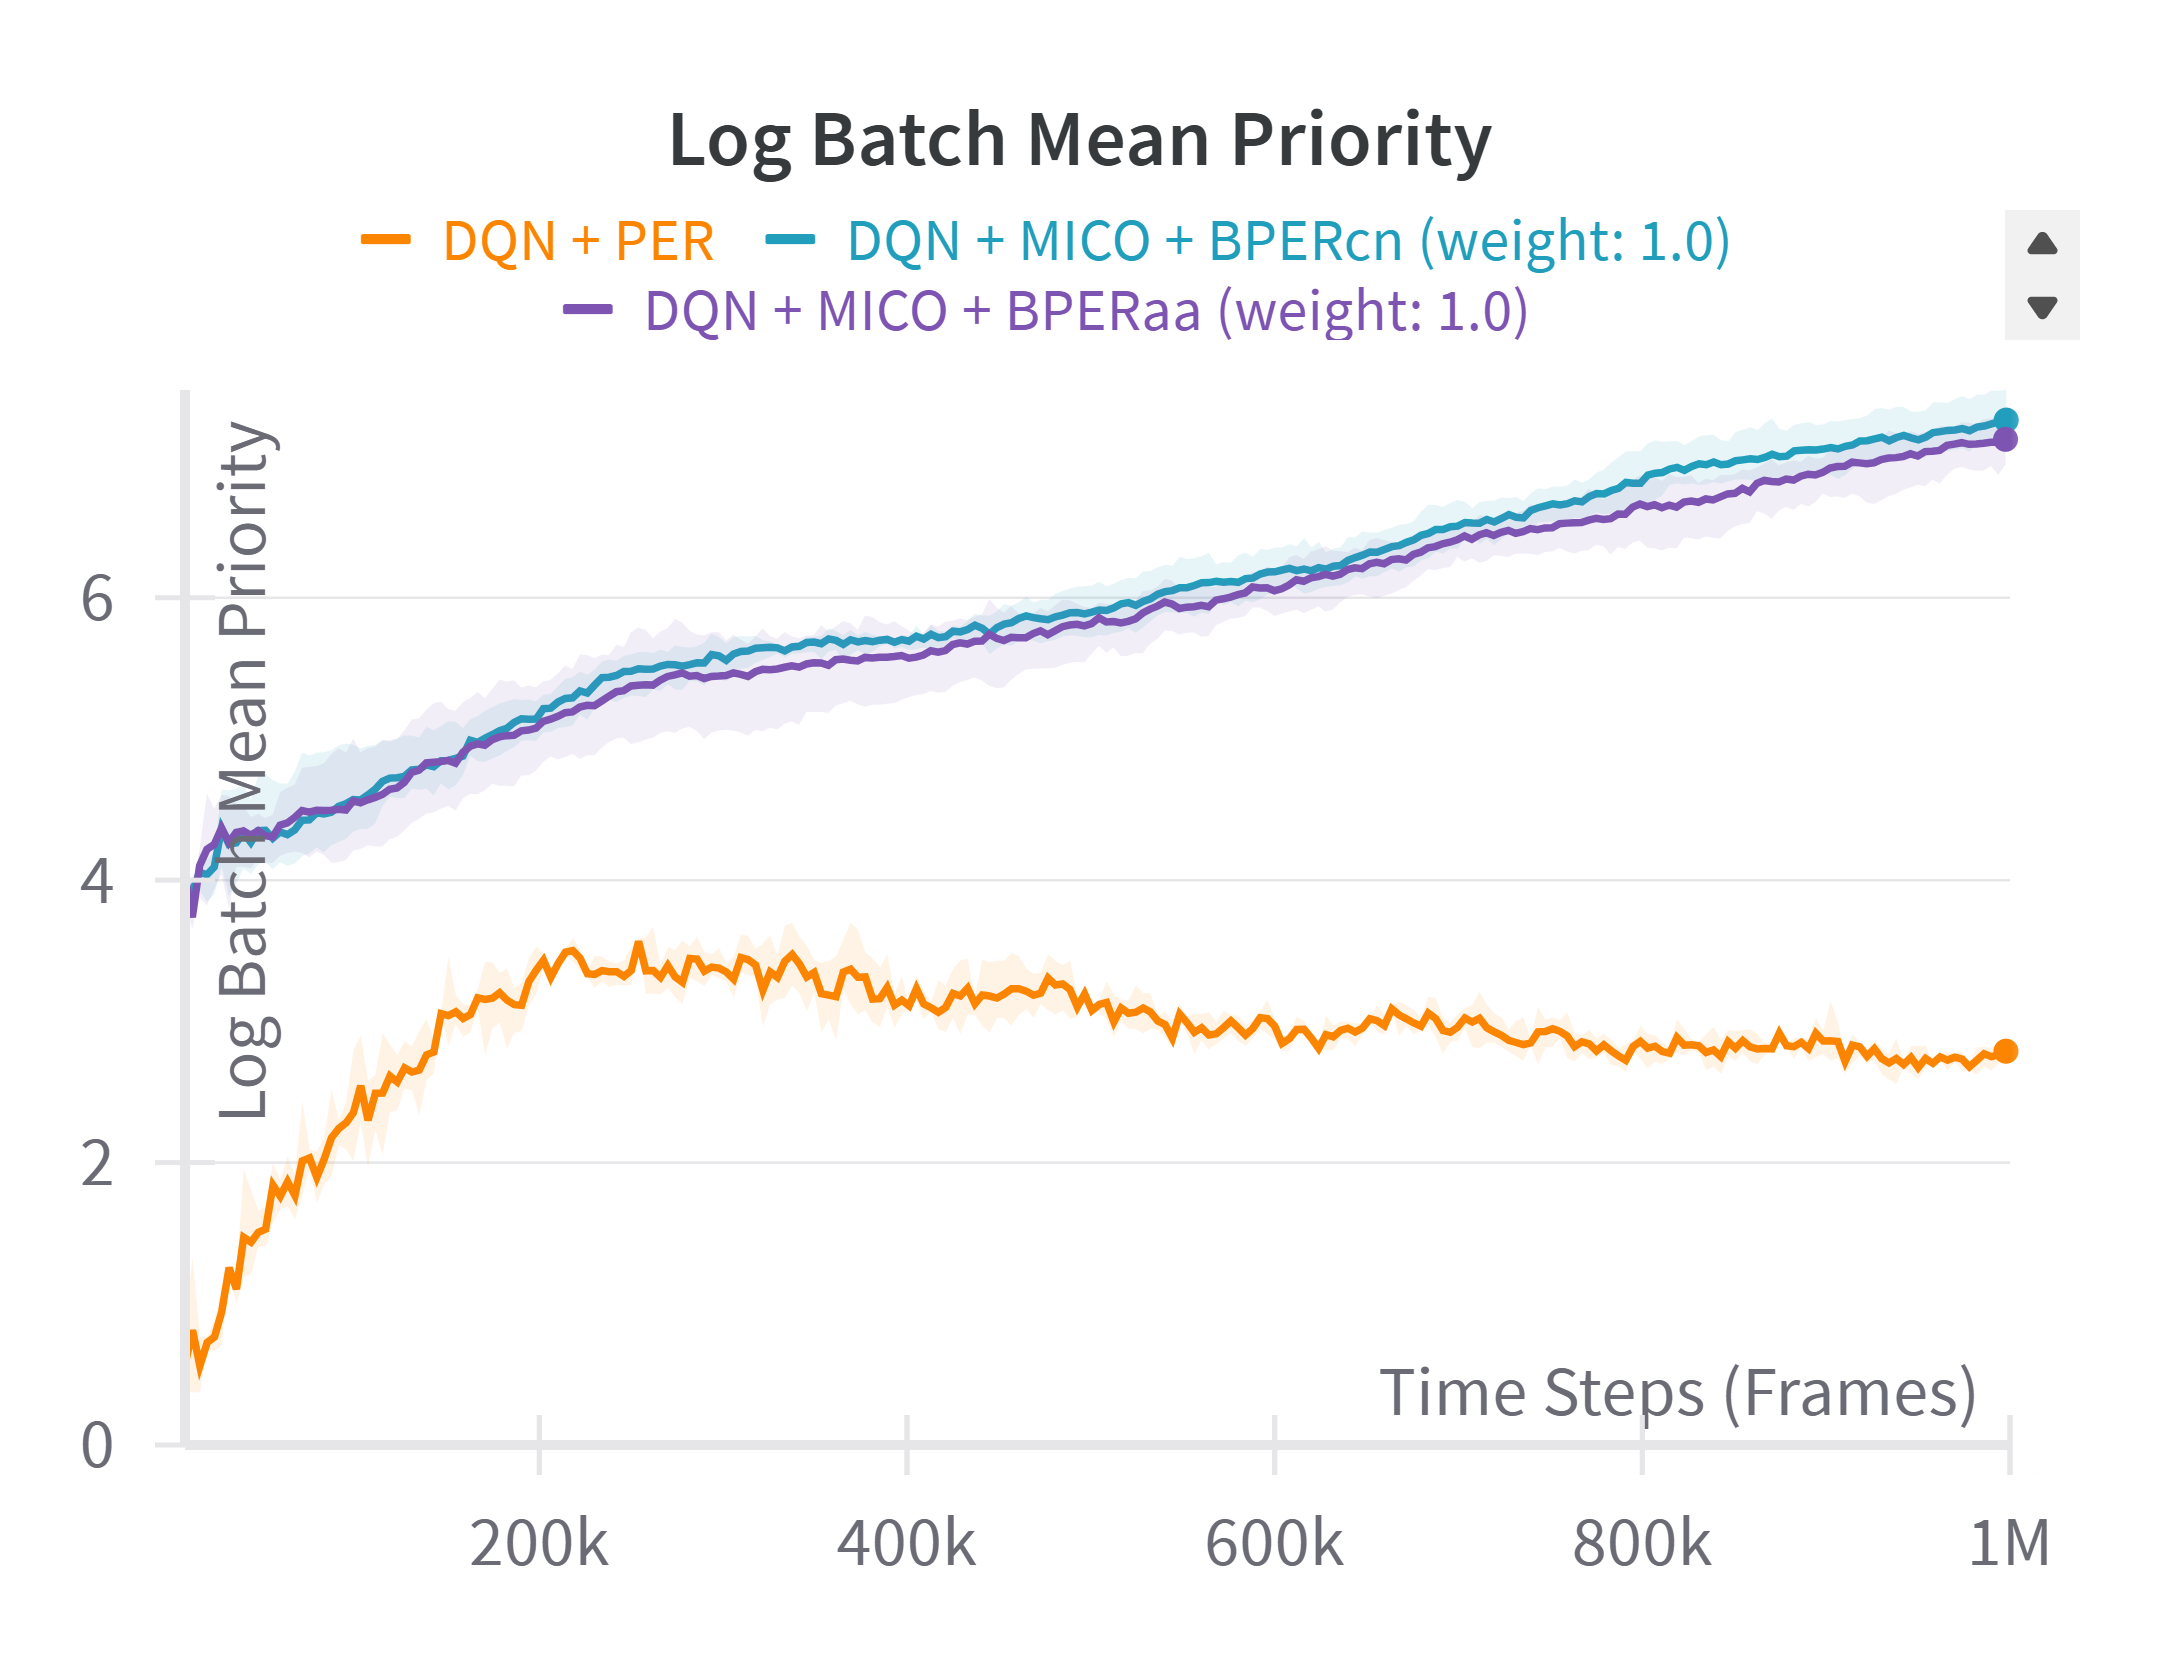
\includegraphics[width=\linewidth]{Results/general_results/log_mean_batch_priority_acrobot.png}
        \caption{Acrobot-v1}
        \label{fig:uniform_weighting}
    \end{subfigure}
    \caption{Two images side-by-side}
    \label{fig:outdated_priorities}
\end{figure}
